%--------------------------------------------------------------------%
%
% Berkas utama templat LaTeX.
%
% author Petra Barus, Peb Ruswono Aryan
%
%--------------------------------------------------------------------%
%
% Berkas ini berisi struktur utama dokumen LaTeX yang akan dibuat.
%
%--------------------------------------------------------------------%
\documentclass[11pt, a4paper, onecolumn, oneside, final]{book}

%-------------------------------------------------------------------%
%
% Konfigurasi dokumen LaTeX untuk laporan tesis IF ITB
%
% @author Petra Novandi
%
%-------------------------------------------------------------------%
%
% Berkas asli berasal dari Steven Lolong
%
%-------------------------------------------------------------------%

% Ukuran kertas
\special{papersize=210mm,297mm}

% Setting margin
\usepackage[top=3cm,bottom=4cm,left=4cm,right=3cm]{geometry}

\usepackage{mathptmx}

% Judul bahasa Indonesia
\usepackage[bahasa]{babel}

% Format citation
%\usepackage[backend=bibtex,citestyle=authoryear]{biblatex}
\usepackage{natbib}

\usepackage[utf8]{inputenc}
\usepackage{csquotes}
\usepackage{graphicx}
\usepackage{titling}
\usepackage{blindtext}
\usepackage{sectsty}
\usepackage{chngcntr}
\usepackage{etoolbox}
\usepackage{hyperref}       % Package untuk link di daftar isi.
\usepackage{titlesec}       % Package Format judul
\usepackage{parskip}
%\usepackage{pgfgantt}
\usepackage{ragged2e}
\usepackage{libertine}
\usepackage{booktabs}
\usepackage{longtable}
\usepackage{array}
\usepackage{caption}
\usepackage{enumitem}
\usepackage{listings}
\usepackage{textcase}
\usepackage{setspace}
\usepackage{afterpage}
\usepackage{multirow}
% \usepackage{tocloft}
\usepackage{amsmath,amsfonts}
\usepackage[table]{xcolor}

\captionsetup[longtable]{skip=0.1em}

% Hypenation
%--------------------------------------------------------------------%
%
% Hypenation untuk Bahasa Indonesia
%
% @author Petra Barus
%
%--------------------------------------------------------------------%
%
% Secara otomatis LaTeX dapat langsung memenggal kata dalam dokumen,
% tapi sering kali terdapat kesalahan dalam pemenggalan kata. Untuk
% memperbaiki kesalahan pemenggalan kata tertentu, cara pemenggalan
% kata tersebut dapat ditambahkan pada dokumen ini. Pemenggalan
% dilakukan dengan menambahkan karakter '-' pada suku kata yang
% perlu dipisahkan.
%
% Contoh pemenggalan kata 'analisa' dilakukan dengan 'a-na-li-sa'
%
%--------------------------------------------------------------------%
% inhyph.tex 
% Version 1.3 19-SEP-1997
%
% Hyphenation patterns for bahasa indonesia (probably also usable
% for bahasa melayu)
%
% (c) Copyright 1996, 1997 J\"org Knappen and Terry Mart
% 
% This patterns are free software according to the GNU General Public 
% licence version 2, June 1991.
%
% Please read the GNU licence for details. If you don't receive a GNU
% licence with these patterns, you can obtain it from 
%
%                          Free Software Foundation, Inc.
%                          675 Mass Ave, Cambridge, MA 02139, USA
%
% If you make any changes to this file, please rename it so that it
% cannot be confused with the original one, and change the contact
% address for bug reports and suggestions.
%
% For bug reports, improvements, and suggestions, contact
%
% J\"org Knappen
% jk Unternehmensberatung
% Barbarossaring 43
% 55118 Mainz
%
% knappen@vkpmzd.kph.uni-mainz.de
%
% or:
% Terry Mart
%
% Institut fuer Kernphysik
% Universitaet Mainz
% 55099 Mainz
% Germany
%
% phone : +49 6131 395174
% fax   : +49 6131 395474
% email : mart@kph.uni-mainz.de
%
%*%*%*%*%*%*%*%*%*%*%*%*%*%*%*%*%*%*%*%*%*%*%*%*%*%*%*%*%*%*%*%*%*%*%*%*%*%*%*%*
%
% The patterns are best used with the following parameters
%
% \lefthyphenmin=2 \righthyphenmin=2 %
%
%*%*%*%*%*%*%*%*%*%*%*%*%*%*%*%*%*%*%*%*%*%*%*%*%*%*%*%*%*%*%*%*%*%*%*%*%*%*%*%*
%
% \patterns{%
% a1 e1 i1 o1 u1 % allow hyphens after vowels
% 2b1d 2b1j 2b1k 2b1n 2b1s 2b1t
% 2c1k 2c1n
% 2d1k 2d1n 2d1p 
% 2f1d 2f1k 2f1n 2f1t
% 2g1g 2g1k 2g1n
% 2h1k 2h1l 2h1m 2h1n 2h1w
% 2j1k 2j1n
% 2k1b 2k1k 2k1m 2k1n 2k1r 2k1s 2k1t
% 2l1b 2l1f 2l1g 2l1h 2l1k 2l1m 2l1n 2l1s 2l1t 2l1q
% 2m1b 2m1k 2m1l 2m1m 2m1n 2m1p 2m1r 2m1s
% 2n1c 2n1d 2n1f 2n1j 2n1k 2n1n 2n1p 2n1s 2n1t 2n1v
% 2p1k 2p1n 2p1p 2p1r 2p1t
% 2r1b 2r1c 2r1f 2r1g 2r1h 2r1j 2r1k 2r1l 2r1m 2r1n 2r1p 2r1r 2r1s 2r1t 2r1w 2r1y
% 2s1b 2s1k 2s1l 2s1m 2s1n 2s1p 2s1r 2s1s 2s1t 2s1w
% 2t1k 2t1l 2t1n 2t1t  
% 2w1t                 % two consonant groups to be hyphenated between
%                      % the consonants
% 2ng1g 2ng1h 2ng1k 2ng1n 2ng1s    % three consonant groups
% 2n3s2t % kon-stan-ta
% .be2r3 .te2r3 .me2ng3 .pe2r3 % prefixes
% 2ng. 2ny. % don't hyphenate -ng and -ny at the end of word
% i2o1n % in-ter-na-sio-nal
% a2ir % ber-air 
% 1ba1ga2i % se-ba-gai-ma-na
% 2b1an. 2c1an. 2d1an. 2f1an. 2g1an. 2h1an. 2j1an. 2k1an. 2l1an.
% 2m1an. 2ng1an. 2n1an. 2p1an. 2r1an. 2s1an. 2t1an. 2v1an. 2z1an. 
% 3an. % suffix -an
% .a2ta2u % atau-pan
% .ta3ng4an. .le3ng4an. .ja3ng4an. .ma3ng4an. .pa3ng4an. .ri3ng4an. 
% .de3ng4an. % Don't overload the exception list...
% }
% Exeptions to the above rules, specially words beginning in ber...
% and ter..
\hyphenation{be-ra-be be-ra-hi be-rak be-ran-da be-ran-dal be-rang
             be-ra-ngas-an be-rang-sang be-ra-ngus be-ra-ni
             be-ran-tak-an be-ran-tam be-ran-tas be-ra-pa be-ras
             be-ren-deng be-re-ngut be-re-rot be-res be-re-wok
             be-ri be-ri-ngas be-ri-sik be-ri-ta be-rok be-ron-dong
             be-ron-tak be-ru-du be-ruk be-run-tun
             peng-eks-por peng-im-por
             te-ra te-rang te-ras te-ra-si te-ra-tai te-ra-wang te-ra-weh
             te-ri-ak te-ri-gu te-rik te-ri-ma te-ri-pang te-ro-bos
             te-ro-bos-an te-ro-mol te-rom-pah te-rom-pet te-ro-pong
             te-ro-wong-an te-ru-buk te-ru-na te-rus te-ru-si}

\endinput

%\hyphenpenalty=5000
%\tolerance=1000
%\lefthyphenmin=2
%\righthyphenmin=2
\hyphenpenalty=10000
\tolerance=1
\lefthyphenmin=99
\righthyphenmin=99
\sloppy

% Line satu setengah spasi
\renewcommand{\baselinestretch}{1.5}

% Kode lebih kecil
\let\OldTexttt\texttt
\renewcommand{\texttt}[1]{\OldTexttt{\footnotesize{#1}}}

% Listing Code thingy
\lstset{frame=tb,
  breaklines=true,
  showstringspaces=false,
  columns=flexible,
  numbers=none,
  commentstyle=\color{dkgreen},
  stringstyle=\color{mauve},
  tabsize=3
}
\renewcommand{\lstlistingname}{Kode}
\newcommand{\listingsfont}{\rmfamily}

% Add comma between Author and Year
%\renewcommand*{\nameyeardelim}{\addcomma\space}

% \renewcommand{\cftsecleader}{\cftdotfill{\cftdotsep}}

% Setting judul
\chapterfont{\centering \Large}
\titleformat{\chapter}[display]
  {\Large\centering\bfseries}
  {\chaptertitlename\ \thechapter}{0pt}
    {\Large\bfseries\uppercase}
\titlespacing*{\chapter}{0pt}{-25pt}{40pt}

% Setting nomor pada subbsubsubbab
\setcounter{secnumdepth}{4}

\titleformat{\paragraph}
{\normalfont\normalsize\bfseries}{\theparagraph}{1em}{}
\titlespacing*{\paragraph}
{0pt}{3.25ex plus 1ex minus .2ex}{1.5ex plus .2ex}

\titlespacing*{\section} {0pt}{2.5ex plus 1ex minus .2ex}{1.3ex plus .2ex}
\titlespacing*{\subsection} {0pt}{2.25ex plus 1ex minus .2ex}{0.5ex plus .2ex}

\makeatletter
\makeatother

% Counter untuk figure dan table.
\counterwithin{figure}{chapter}
\counterwithin{table}{chapter}

% For Gantt Chart
\newcounter{myWeekNum}
\stepcounter{myWeekNum}
%
\newcommand{\myWeek}{\themyWeekNum
    \stepcounter{myWeekNum}
    \ifnum\themyWeekNum=53
         \setcounter{myWeekNum}{1}
    \else\fi
}
%
\newcolumntype{L}[1]{>{\raggedright\let\newline\\\arraybackslash\hspace{0pt}}m{#1}}
\newcolumntype{C}[1]{>{\centering\let\newline\\\arraybackslash\hspace{0pt}}m{#1}}
\newcolumntype{R}[1]{>{\raggedleft\let\newline\\\arraybackslash\hspace{0pt}}m{#1}}

\makeatletter
\def\@chapter[#1]#2{\ifnum \c@secnumdepth >\m@ne
                         \refstepcounter{chapter}%
                         \typeout{\@chapapp\space\thechapter.}%
                         \addcontentsline{toc}{chapter}%
                                   {\protect{BAB \numberline{\thechapter}\texorpdfstring{\uppercase{#1}}{#1}}}%
                    \else
                      \addcontentsline{toc}{chapter}{\texorpdfstring{\uppercase{#1}}{#1}}%
                    \fi
                    \chaptermark{#1}%
                    \addtocontents{lof}{\protect\addvspace{10\p@}}%
                    \addtocontents{lot}{\protect\addvspace{10\p@}}%
                    \if@twocolumn
                      \@topnewpage[\@makechapterhead{#2}]%
                    \else
                      \@makechapterhead{#2}%
                      \@afterheading
                    \fi}
\makeatother

\makeatletter

\makeatother

%\bibliography{references}

\begin{document}

    %Basic configuration
    \title{Optimasi Pencocokan Pola dalam Sistem Deteksi Intrusi Snort Menggunakan GPU}
    \date{}
    \author{
        AFRIZAL FIKRI \\
        NIM : 13513004
    }

    \frontmatter
    \clearpage
\pagestyle{empty}

\begin{center}
\smallskip

    \Large \bfseries \MakeUppercase{\thetitle}
    \vfill

    \Large Laporan Tugas Akhir
    \vfill

    \large Disusun sebagai syarat kelulusan tingkat sarjana

    \vfill

    \large Oleh

    \Large \theauthor

    \vfill
    \begin{figure}[h]
        \centering
      	
\includegraphics[width=0.15\textwidth]{resources/cover-ganesha}
    \end{figure}
    \vfill

    \large
    \uppercase{
        Program Studi Teknik Informatika \\
        Sekolah Teknik Elektro dan Informatika \\
        Institut Teknologi Bandung
    }

    Agustus 2018

\end{center}

\clearpage

    \clearpage
\pagestyle{empty}

\begin{center}
\smallskip

    \Large \bfseries \MakeUppercase{\thetitle}
    \vfill

    \Large Laporan Tugas Akhir I
    \vfill

    \large Oleh

    \Large \theauthor

    \large Program Studi Teknik Informatika \\
    Sekolah Teknik Elektro dan Informatika \\
    Institut Teknologi Bandung \\

    \vfill
    \normalsize \normalfont
    Bandung, 20 Desember 2016 \\
    Mengetahui, \\~\\    

    \setlength{\tabcolsep}{12pt}
    \begin{tabular}{c@{\hskip 0.5in}c}
        Pembimbing I, & Pembimbing II \\
        & \\
        & \\
        & \\
        & \\
        \underline{Achmad Imam Kistijantoro, S.T., M.Sc, Ph.D} & \underline{Nama dan Gelar Pembimbing II} \\
        NIP. 19730809 200604 1 001 & NIP. 123456789 \\
    \end{tabular}

\end{center}
\clearpage

    \chapter*{Lembar Pernyataan}

Dengan ini saya menyatakan bahwa:

\begin{enumerate}

    \item Pengerjaan dan penulisan Laporan Tugas Akhir ini dilakukan tanpa menggunakan bantuan yang tidak dibenarkan.
    \item Segala bentuk kutipan dan acuan terhadap tulisan orang lain yang digunakan di dalam penyusunan laporan tugas akhir ini telah dituliskan dengan baik dan benar.
    \item Laporan Tugas Akhir ini belum pernah diajukan pada program pendidikan di perguruan tinggi mana pun.

\end{enumerate}

Jika terbukti melanggar hal-hal di atas, saya bersedia dikenakan sanksi sesuai dengan Peraturan Akademik dan Kemahasiswaan Institut Teknologi Bandung bagian Penegakan Norma Akademik dan Kemahasiswaan khususnya Pasal 2.1 dan Pasal 2.2.
\vspace{15mm}

Bandung, 6 Desember 2016 \\
\theauthor


    \pagestyle{plain}

    %\chapter*{ABSTRAK}
\addcontentsline{toc}{chapter}{ABSTRAK}

\begin{center}
\MakeTextUppercase{\textbf{\large{\thetitle}}}

Oleh

\MakeTextUppercase{\theauthor}
\end{center}
\medskip
\begin{spacing}{1.0}

Saat ini, banyak transaksi penting terjadi dunia maya. Keamanan informasi menjadi jaminan yang sangat penting agar data-data penting tidak bocor dan disalahgunakan. Sistem deteksi dan pencegahan intrusi telah dikembangkan. Namun, kecepatan deteksi intrusi belum secepat peningkatan kecepatan jaringan.

Solusi yang dapat digunakan yaitu penggunaan \emph{multithread} untuk pencocokan yang banyak secara paralel. Solusi \emph{multithreading} telah dikembangkan menggunakan CPU. Namun, CPU memiliki \emph{core} yang sangat terbatas. Alternatif lainnya adalah dengan menggunakan GPU. GPU memiliki kemampuan untuk membangkitkan banyak \emph{thread} sekaligus. GPU sangat cocok untuk melakukan komputasi sederhana dalam jumlah besar. 

Salah satu komponen penting dalam sistem deteksi intrusi yaitu pencocokan string. Beban pencocokan string ini seringkali menjadi \emph{bottleneck} dalam analisis paket jaringan. Tugas akhir ini akan mencoba melakukan eksperimen untuk melakukan implementasi pencocokan string pada sistem deteksi intrusi Snort menggunakan GPU.

Untuk dapat mempercepat proses analisis menggunakan GPU, translasi solusi yang ada tidaklah cukup. Operasi dalam GPU seringkali adalah operasi yang I/O \emph{bound} dan \emph{memory bound}. Diperlukan beberapa pengubahan seperti alokasi \emph{thread} yang berbeda, metode transfer memori \emph{host} dan \emph{device}, skema penampungan paket, dan pengubahan struktur data \emph{state machine}. Implementasi dapat menghasilkan \emph{speedup} yang signifikan hingga 3x lipat solusi \emph{multithreading} dengan CPU.

Kata kunci: \textit{pattern matching}, deteksi intrusi, GPU, optimasi, paralel.


\end{spacing}

\clearpage
    % \clearpage
\chapter*{Abstract}
\addcontentsline{toc}{chapter}{Abstract}

%put your abstract here
\blindtext

\clearpage
    \chapter*{Kata Pengantar}
\addcontentsline{toc}{chapter}{KATA PENGANTAR}

Puji dan syukur penulis panjatkan ke hadirat Tuhan yang Maha Esa karena atas berkat dan pertolongan-Nya, penulis dapat menyelesaikan Tugas Akhir dan laporan tugas akhir yang berjudul "\thetitle" ini dengan baik. 

Dalam penyusunan Tugas Akhir ini penulis banyak mendapatkan masukan, kritik, dorongan, bantuan, bimbingan, serta dukungan baik secara fisik maupun moral dari berbagai pihak yang merupakan pengalaman yang berharga yang tidak dapat diukur secara materi dan dapat menjadi pembelajaran yang berharga dikemudian hari. Oleh karena itu dengan segala hormat dan kerendahan hati perkenankanlah penulis mengucapkan terima kasih kepada:

\begin{enumerate}
    \item Bapak Achmad Imam Kistijantoro, S.T., M.Sc., Ph.D. selaku pembimbing penulis atas ilmu yang diberikan selama bimbingan maupun perkuliahan, kritik dan saran, serta dukungan moral yang diberikan selama proses pengerjaan tugas akhir.

    \item Bapak Yudistira Dwi Wardhana Asnar, Ph.D selaku penguji atas saran dan masukkannya sehingga membuat Tugas Akhir ini menjadi lebih baik.

    \item Kedua orang tua penulis. Terima kasih atas dukungan baik secara moral dan material sehingga penulis dapat melaksanakan Tugas Akhir ini hingga selesai dengan baik.
    
    \item Ibu Dr. Fazat Nur Azizah ST, M.Sc. selaku dosen Tugas Akhir yang telah memotivasi saya dan memberikan arahan dalam penyelesaian dan pengerjaan Tugas Akhir ini.
    
    % \item Ibu Dr. Eng. Ayu Purwarianti, ST., MT. selaku dosen mentor Imagine Cup yang ikut membantu dan memberikan dukungan agar penulis dapat menyelesaikan pengerjaan Tugas Akhir.
    
	% \item Bapak Dr.techn. Saiful Akbar ST, MT. dan Bapak Achmad Imam Kistijantoro, ST, M.Sc, Ph.D selaku Ketua Program Studi dari Teknik Informatika dan Sistem dan Teknologi Informasi yang ikut mendukung penulis dalam menyelesaikan Tugas Akhir ini.
    
    \item Seluruh dosen, karyawan dan civitas program studi Teknik Informatika, Institut Teknologi Bandung.
    
    \item Rekan-rekan yang telah penulis minta bantuan dalam penyelesaian administrasi Tugas Akhir ini disaat penulis berhalangan terutama Muhamad Visat Sutarno dan Fiqie Ulya Sidiastahta
    
    % \item Rekan-rekan laboratorium basis data yang saling mendukung dalam menyelesaikan Tugas Akhir ini pada khususnya Vanya Deasy Safrina, Albert Tri Adrian, Marco Orlando, Fiqie Ulya Sidiastahta, dan Wilhelmus Andrian.
    
    \item Rekan-rekan seperjuangan Teknik Informatika yang menamakan dirinya Happy Anti Wacana yang selalu mendukung penulis untuk mengerjakan Tugas Akhir.
    
    \item Rekan-rekan dari Binary 2013 dan HMIF yang telah memberikan dukungan dan bantuan dalam pengerjaan Tugas Akhir.
    
    \item Pihak-pihak lain yang tidak dapat disebutkan satu-persatu.
\end{enumerate}

Penulis menyadari bahwa Tugas Akhir ini masih jauh dari sempurna serta memiliki banyak kekurangan. Oleh karena itu, penulis sangat terbuka dalam menerima kritik dan saran yang membangun untuk Tugas Akhir ini. Semoga Tugas Akhir ini dapat bermanfaat bagi pembaca.

\begin{flushright}
Bandung, September 2018 \\
\vspace{25mm}
Penulis
\end{flushright}



    \titleformat*{\section}{\centering\bfseries\Large\MakeUpperCase}
    
    \tableofcontents
    \addcontentsline{toc}{chapter}{DAFTAR ISI} 
    % \afterpage{\null\newpage}
    % \addcontentsline{toc}{chapter}{DAFTAR LAMPIRAN}
    {%
        \let\oldnumberline\numberline%
        \renewcommand{\numberline}{\figurename~\oldnumberline}%
        \listoffigures%
    }
    \addcontentsline{toc}{chapter}{DAFTAR GAMBAR}  
    {%
        \let\oldnumberline\numberline%
        \renewcommand{\numberline}{\tablename~\oldnumberline}%
        \listoftables%
    }
    \addcontentsline{toc}{chapter}{DAFTAR TABEL}

    %----------------------------------------------------------------%
    % Konfigurasi Bab
    %----------------------------------------------------------------%
    \renewcommand{\chaptername}{BAB}
    \renewcommand{\thechapter}{\Roman{chapter}}
    %----------------------------------------------------------------%

    \titleformat*{\section}{\bfseries\large}
    \mainmatter
    %----------------------------------------------------------------%
    % Dafter Bab
    % Untuk menambahkan daftar bab, buat berkas bab misalnya `chapter-6` di direktori `chapters`, dan masukkan ke sini.
    %----------------------------------------------------------------%
    %!TeX root=../thesis.tex

\chapter{Pendahuluan}

  % Pada bab ini akan dibahas mengenai landasan dari pelaksanaan Tugas Akhir tentang sistem deteksi intrusi jaringan.

\section{Latar Belakang}

  Penjaminan keamanan informasi merupakan cara-cara untuk mencegah pengaksesan, penggunaan, penyebaran, pengubahan, penyalinan, atau perusakan data yang tidak berhak. Beberapa aspek yang penting untuk dijamin dalam sebuah informasi adalah \emph{confidentiality}, \emph{integrity} dan \emph{availability}. Ketiganya biasa disebut CIA Triad dan telah menjadi pedoman prinsip keamanan informasi yang dikenal luas \citep{nist2003}. Pada tahun 1998, Donn Parker mengusulkan aspek tambahan penjaminan informasi yaitu \emph{possession}, \emph{authenticity}, dan \emph{utility} \citep{parker1998}. Parker berpendapat bahwa model CIA hanya berfokus pada aset saja tidak pada kontrol pengguna.

  Pengamanan dapat dilakukan pada 2 sisi sumber daya, yaitu \emph{tangible resources} dan \emph{intangible resources}. \emph{Tangible resources} yaitu aset yang berupa barang kasar (yang memiliki rupa). Contoh \emph{tangible resources} misal \emph{client}, \emph{server}, dan \emph{channel} komunikasi (komunikasi kabel dan nirkabel). \emph{Intangible resources} yaitu aset yang tidak memiliki rupa, yaitu isi dari informasi yang dikirimkan. Baik keamanan dari \emph{tangible resources} maupun \emph{intangible resources} saling terkait dan memiliki peran penting dalam menjamin aset yang lain \citep{kizza2015}.

  Salah satu sumber daya yang penting untuk dilindungi yaitu \emph{server}. Banyak aspek security yang terdapat pada \emph{server} dan dapat dengan mudah diserang \citep{owasp}. Solusi untuk pengamanan \emph{server} dari \emph{request} berbahaya adalah dengan menggunakan sistem deteksi intrusi jaringan (\emph{network intrusion detection system} abbr. NIDS). NIDS berfungsi mengenali kemungkinan serangan dari \emph{request} yang diterima pada \emph{server} atau \emph{client} sebagai tindakan pencegahan. Ketika \emph{request} dianggap berbahaya, maka dapat dilakukan tindakan lanjutan untuk mencegah kerusakan lebih lanjut pada aset. NIDS yang melakukan tindakan preventif seperti ini disebut juga NIPS (\emph{network intrusion prevention system}).

  Salah satu contoh NIDS yang banyak digunakan adalah NIDS Snort. Snort adalah salah satu NIDS berbasis \emph{signature} yang mencocokan paket dengan \emph{rule} yang telah dikumpulkan. \emph{Rule} Snort terdiri dari beberapa komponen yang bertujuan mengenali \emph{host} asal, \emph{host} tujuan, dan isi paket jaringan. \emph{Rule} yang digunakan berasal dari riset para pakar keamanan dan terus diperbaharui mengikuti pola-pola serangan terbaru.

  Karena adanya peningkatan kecepatan \emph{traffic} internet dan banyaknya serangan yang terjadi, maka dibutuhkan NIDS yang mampu melakukan deteksi dengan lebih cepat. Salah satu \emph{bottleneck} dalam pengecekan paket adalah banyaknya \emph{rule} yang harus dicocokkan \citep{pcre2007}. Sehingga, peningkatan secara signifikan dapat dicapai salah satunya dengan meningkatkan kemampuan komputasi untuk pencocokan banyak paket secara paralel. Pemanfaatan \emph{multithreading} pada \emph{multicore processor} telah dikembangkan untuk mempercepat kinerja NIDS \citep{multi2004}.

  Selain mengoptimalkan penggunaan CPU, alternatif yang dapat digunakan yaitu penggunaan \emph{general purpose} GPU (GPGPU) \citep{4482891}. Dapat juga menggunakan prosesor yang mudah dikustomisasi seperti ASIC atau FPGA \citep{fpga2008}. GPGPU banyak digunakan karena perangkat yang mudah didapatkan, multiguna, dan hanya membutuhkan lebih sedikit kustomisasi daripada ASIC dan FPGA. Selain itu, perbandingan kinerja antara GPGPU dan ASIC atau FPGA tidak terlalu jauh tanpa melakukan kustomisasi lebih lanjut di tingkat \emph{low level} \citep{gnort2008}. Maka, Tugas Akhir ini akan fokus untuk melakukan pembangunan NIDS yang berbasis GPGPU.

\section{Rumusan Masalah}

  Melakukan pencocokan pola secara paralel memiliki beberapa masalah yaitu algoritma yang digunakan, penyimpanan \emph{dictionary}, dan metode \emph{streaming} paket. Dan juga hasil yang diharapkan dapat menangani kasus dengan kapasitas aliran data yang besar. Maka dari itu, Tugas Akhir ini akan difokuskan pada pembangunan sistem deteksi intrusi jaringan paralel dengan GPU. Dalam rangka pembangunan sistem tersebut, terdapat beberapa permasalahan yang menjadi fokus perhatian dari penelitian ini, yaitu: 

  \begin{enumerate}
      \item Bagaimana arsitektur yang memadai terkait pencocokan pola dengan GPU?
      \item Bagaimana kinerja sistem deteksi intrusi jaringan akibat dari penggunaan GPU?
  \end{enumerate}

\section{Tujuan}

  Tujuan dari pelaksanaan Tugas Akhir ini adalah sebagai berikut:
  \begin{enumerate}
      \item Mengembangkan sebuah arsitektur yang memadai untuk pencocokan pola dengan GPU
      \item Melakukan perbandingan kinerja sistem deteksi intrusi jaringan sebelum dan setelah menggunakan GPU
  \end{enumerate}

\section{Batasan Masalah}

  Merancang NIDS yang cepat dengan menggunakan GPU merupakan solusi yang cocok untuk menghadapi serangan yang semakin meningkat. Tugas Akhir ini akan difokuskan pada pembangunan sistem yang melakukan inspeksi paket secara cepat menggunakan komputasi paralel pada GPU. Dalam rangka pembangunan sistem tersebut, terdapat beberapa batasan yang digunakan dalam penelitian ini, yaitu:
  \begin{enumerate}
      \item NIDS dibuat di atas NIDS Snort
      \item NIDS menggunakan \emph{platform} GPGPU CUDA
      \item \emph{Payload} akan diambil dari \emph{log} jaringan berupa berkas PCAP
      \item NIDS menggunakan \emph{rule} milik Snort VRT yang disesuaikan
  \end{enumerate}

\section{Metodologi}

  Tahapan yang akan dilakukan selama pelaksanaan Tugas Akhir ini adalah sebagai berikut:
  \begin{enumerate}

      \item Analisis Permasalahan \\
      Pengerjaan Tugas Akhir ini diawali dengan analisis terhadap permasalahan yang ingin diteliti lebih lanjut. Pada tahap ini, studi literatur perlu dilakukan dalam rangka mempelajari hasil-hasil penelitian terkait yang telah dilakukan, berikut metodologi penelitian serta ketercapaian yang berhasil didapatkan. Selain itu, tahap ini juga menjadi langkah awal untuk merumuskan landasan teori, penarikan hipotesis, hingga akhirnya dicapai rancangan solusi yang akan digunakan untuk membangun sistem deteksi intrusi.

      \item Analisis Metode \\
      Pada tahap analisis metode, dilakukan eksplorasi yang bertujuan untuk mendapatkan metode-metode terbaik yang dapat digunakan sebagai komponen dalam pencocokan \emph{signature}. Analisis yang dilakukan mencakup memori \emph{layout} untuk \emph{dictionary}, dan algoritma pencocokan \emph{signature}. Selain dilakukan eksperimen secara umum dengan mengacu pada penelitian-penelitian serupa yang pernah dilakukan sebelumnya, akan dilakukan pula eksperimen dengan beberapa modifikasi yang dianggap perlu.

      \item Implementasi Sistem \\
      Pembangunan sistem deteksi intrusi dilakukan dengan memanfaatkan hasil yang didapatkan dari tahapan sebelumnya, yakni metode-metode dan algoritma pencocokan pola.

      \item Evaluasi dan Penarikan Kesimpulan \\
      Pada tahap ini dilakukan evaluasi terhadap sistem deteksi intrusi yang telah dibangun. Selain itu, dilakukan juga penarikan kesimpulan yang didasari oleh hasil evaluasi pengujian sistem deteksi intrusi.

  \end{enumerate}

%\section{Jadwal Pelaksanaan Tugas Akhir}

%  Berikut adalah rencana kegiatan dan jadwal (dirinci sampai per minggu) mulai dari awal pelaksanaan Tugas Akhir I s.d. sidang Tugas Akhir beserta \emph{milestones} dan \emph{deliverables}. \\
%  \begin{figure}[H]
\begin{ganttchart}[
  y unit title=0.6cm,
  y unit chart=1.5cm,
  x unit=1.2mm,
  vgrid={*{6}{draw=none},dotted},
  hgrid,
  title label anchor/.style={below=-1.6ex},
  title left shift=.05,
  title right shift=-.05,
  title height=1,
  bar label node/.style={text width=2cm, align=right, font=\scriptsize\RaggedLeft, anchor=east},
  incomplete/.style={fill=white},
  progress label text={},
  bar height=.4,
  group right shift=0,
  group top shift=0,
  group height=.3,
  group peaks height=.2,
  time slot format=isodate,
  time slot format/start date=2017-02-1
]{2017-03-01}{2017-05-31}

\ganttset{calendar week text=\currentweek}

%labels
\gantttitlecalendar{year, month=shortname, week=1} \\

%tasks
\ganttbar{Analisis Permasalahan}{2017-03-06}{2017-05-07} \\
\ganttbar{Analisis Metode}{2017-05-01}{2017-05-31} \\
\ganttbar{Implementasi Sistem}{2017-08-06}{2017-10-14} \\
\ganttbar{Evaluasi dan Penarikan Kesimpulan}{2017-10-14}{2018-01-10}

%relations
% \ganttlink{elem0}{elem1} %
% \ganttlink{elem1}{elem2} %
% \ganttlink{elem2}{elem3} %

\end{ganttchart}

\end{figure}

\begin{figure}[H]
\begin{ganttchart}[
  y unit title=0.6cm,
  y unit chart=1.5cm,
  x unit=1.5mm,
  vgrid={*{6}{draw=none},dotted},
  hgrid,
  title label anchor/.style={below=-1.6ex},
  title left shift=.05,
  title right shift=-.05,
  title height=1,
  bar label node/.style={text width=2cm, align=right, font=\scriptsize\RaggedLeft, anchor=east},
  incomplete/.style={fill=white},
  progress label text={},
  bar height=.4,
  group right shift=0,
  group top shift=0,
  group height=.3,
  group peaks height=.2,
  time slot format=isodate,
  time slot format/start date=2017-02-1
]{2017-06-01}{2017-08-31}

\ganttset{calendar week text=\currentweek}

%labels
\gantttitlecalendar{year, month=shortname, week=14} \\

%tasks
\ganttbar{Analisis Permasalahan}{2017-03-05}{2017-03-06} \\
\ganttbar{Analisis Metode}{2017-06-01}{2017-08-27} \\
\ganttbar{Implementasi Sistem}{2017-08-07}{2017-08-31} \\
\ganttbar{Evaluasi dan Penarikan Kesimpulan}{2017-10-14}{2018-01-10}

%relations
% \ganttlink{elem0}{elem1} %
% \ganttlink{elem1}{elem2} %
% \ganttlink{elem2}{elem3} %

\end{ganttchart}

\end{figure}

\begin{figure}[H]
\begin{ganttchart}[
  y unit title=0.6cm,
  y unit chart=1.5cm,
  x unit=1.2mm,
  vgrid={*{6}{draw=none},dotted},
  hgrid,
  title label anchor/.style={below=-1.6ex},
  title left shift=.05,
  title right shift=-.05,
  title height=1,
  bar label node/.style={text width=2cm, align=right, font=\scriptsize\RaggedLeft, anchor=east},
  incomplete/.style={fill=white},
  progress label text={},
  bar height=.4,
  group right shift=0,
  group top shift=0,
  group height=.3,
  group peaks height=.2,
  time slot format=isodate,
  time slot format/start date=2017-02-1
]{2017-09-01}{2017-11-30}

\ganttset{calendar week text=\currentweek}

%labels
\gantttitlecalendar{year, month=shortname, week=27} \\

%tasks
\ganttbar{Analisis Permasalahan}{2017-03-05}{2017-05-06} \\
\ganttbar{Analisis Metode}{2017-04-30}{2017-06-19} \\
\ganttbar{Implementasi Sistem}{2017-09-01}{2017-10-15} \\
\ganttbar{Evaluasi dan Penarikan Kesimpulan}{2017-10-16}{2017-11-30}

%relations
% \ganttlink{elem0}{elem1} %
% \ganttlink{elem1}{elem2} %
% \ganttlink{elem2}{elem3} %

\end{ganttchart}

\caption{\emph{Gantt chart} pelaksanaan tugas akhir}
\end{figure}


%  Adapun penjelasan lebih rinci untuk jadwal pelaksanaan Tugas Akhir I hingga sidang Tugas Akhir dapat dilihat pada tabel berikut. \\
%  \begin {table}[H]
\begin{center}
\begin{tabular}{|p{.5cm}|l|l|l|l|}

\hline
No & Kegiatan & \multicolumn{2}{|l|}{Waktu Pengerjaan} & \\
\hline

1 & \multirow{13}{2.5cm}{Studi literatur mengenai penelitian terkait} & \multirow{4}{*}{Maret 2017} & Minggu ke-1 & - \\
\cline{1-1} \cline{4-5}

2 & & & Minggu ke-2 & - \\
\cline{1-1} \cline{4-5}

3 & & & Minggu ke-3 & - \\
\cline{1-1} \cline{4-5}

4 & & & Minggu ke-4 & - \\
\cline{1-1} \cline{4-5}

5 & & & Minggu ke-5 & - \\
\cline{1-1} \cline{3-5}

6 & & \multirow{4}{*}{April 2017} & Minggu ke-6 & - \\
\cline{1-1} \cline{4-5}

7 & & & Minggu ke-7 & \emph{Draft} Bab I \\
\cline{1-1} \cline{4-5}

8 & & & Minggu ke-8 & - \\
\cline{1-1} \cline{4-5}

9 & & & Minggu ke-9 & \emph{Draft} Bab II \\
\cline{1-1} \cline{4-5}

10 & & \multirow{4}{*}{Mei 2017} & Minggu ke-10 & Revisi Bab II \\
\cline{1-1} \cline{3-5}

11 & & & Minggu ke-11 & \emph{Draft} Bab III \\
\cline{1-1} \cline{4-5}

12 & & & Minggu ke-12 & Revisi Bab III \\
\cline{1-1} \cline{4-5}

13 & & & Minggu ke-13 & Revisi Bab II dan III \\
\hline

\end{tabular}
\caption {\emph{Deliverables} tahapan pengerjaan tugas akhir}
\end{center}
\end{table}


    %!TeX root=../thesis.tex

\chapter{Studi Literatur}

  Pada bab ini akan dipaparkan mengenai beberapa penelitian terkait deteksi intrusi paralel berbasis GPU yang telah dilakukan sebelumnya berikut metodologi serta ketercapaian yang didapatkan. Selain itu, pada bab ini juga akan dijelaskan lebih lanjut mengenai landasan teori dari pengerjaan tugas ini.


\section{Deteksi dan Pencegahan Intrusi}

  \subsection{Deteksi Intrusi}

    Intrusi merupakan serangkaian percobaan yang tidak berhak, baik sukses maupun tidak, untuk menyusup masuk, mengakses, mengubah, atau menyalahgunakan sumber daya yang berharga sehingga sumber daya menjadi tidak dapat dipercaya atau bahkan digunakan \citep{kizza2015}. Proses intrusi sistem terbagi menjadi beberapa tahap. Proses dimulai dengan identifikasi target. Lalu target akan diperiksa secara menyeluruh dan dicari celah keamanannya. Selanjutnya dilakukan pengambilalihan akses ke sistem. Dan terakhir, sumber daya dalam sistem dapat dibaca, digunakan dan dimodifikasi. 

    Deteksi intrusi adalah kegiatan merekam, menganalisa, dan mendeteksi kemungkinan sebuah percobaan akses yang tidak berhak terhadap sebuah sistem \citep{kizza2015}. Adanya percobaan akses ilegal dapat mengindikasikan adanya serangan dari luar (\emph{hijacking}), maupun dari dalam (seperti \emph{malware}). Setelah serangan ditemukan, aktivitas akan dicatat ke log untuk ditindak lebih lanjut.

    Selain deteksi intrusi, kegiatan yang berkaitan adalah pencegahan intrusi. Pencegahan intrusi merupakan deteksi intrusi yang secara aktif melakukan penyaringan terhadap percobaan akses ke sistem. Jika terindikasi sistem terkena percobaan serangan, maka semua percobaan akses yang terkait akan dihentikan. Tindakan lebih lanjut yaitu aliran paket bisa diblok baik untuk sementara waktu maupun secara permanen.

  \subsection{Sistem Deteksi dan Pencegahan Intrusi}

    Sistem deteksi dan pencegahan intrusi (\emph{intrusion detection and prevention system} abbr IDPS) adalah mekanisme yang mengotomasi proses deteksi dan pencegahan intrusi kepada satu atau beberapa node. Sistem mengambil paket yang masuk sambil melakukan pengecekan kemudian membuat laporan hasil inspeksi. Laporan hasil inspeksi dapat digunakan untuk menentukan aksi yang akan dilakukan pada paket \citep{nist2007}.

    Ada dua macam NIDPS dilihat dari cakupan deteksinya:
    \begin{enumerate}

      \item 
      \emph{Network Based IDPS (NIDPS)} \\
      IDPS tipe ini dapat melakukan analisis aliran paket dalam suatu subnet jaringan. IDPS ini biasanya diletakkan di sebuah segment jaringan seperti \emph{gateway}, \emph{hub / switch}, \emph{router}, dsb. Cara kerja NIDPS mirip dengan \emph{network sniffer}, yaitu mengambil seluruh paket yang berjalan pada jaringan. IDPS jenis ini digunakan untuk mengantisipasi serangan jenis DoS (\emph{denial of service}) dan \emph{network probing}.

       \item 
      \emph{Host Based IDPS (HIDPS)} \\
      IDPS tipe ini dapat mengambil seluruh informasi pada sistem operasi seperti \emph{audit trails}, \emph{logs}, \emph{system logs}, dsb dan melakukan analisis terhadap perilaku sistem. IDPS jenis ini digunakan untuk mengantisipasi serangan yang menargetkan sistem operasi, seperti \emph{buffer overflow}, \emph{malware}, dll.

    \end{enumerate}

    Fokus tugas akhir ini akan membahas tentang NIDPS.

  \subsection{Metode Deteksi Intrusi}

    Ada tiga macam metode deteksi yang biasa dipakai dalam NIDPS:
    \begin{enumerate}

      \item
      \emph{Signature-based Detection} \\
      \emph{Signature} adalah pola aktivitas tertentu yang mengindikasikan adanya ancaman. IDS berbasis \emph{signature} melakukan pencocokan \emph{signature} dengan aktivitas sistem untuk mengidentifikasi insiden yang mungkin. Pengenalan berbasis \emph{signature} sangat efektif dan cepat untuk mendeteksi ancaman yang telah dikenal. Tapi metode ini tidak efektif untuk mendeteksi ancaman yang belum pernah dikenal sebelumnya atau ancaman yang disamarkan dengan teknik-teknik tertentu.

      Metode ini adalah metode termudah karena hanya membandingkan unit aktivitas saat ini, seperti paket atau \emph{log entry}, dengan daftar \emph{signature} menggunakan operasi perbandingan string. Selain itu jumlah \emph{false alarm} yang dihasilkan juga relatif sedikit. Metode berbasis \emph{signature} membutuhkan sedikit pengetahuan tentang protokol jaringan dan aplikasi, dan tidak dapat melacak atau mendapat state dari komunikasi yang kompleks.

      \item
      \emph{Anomaly-based Detection} \\
      IDS berbasis anomali melakukan analisis parameter aktivitas yang dianggap normal dengan aktivitas sistem sekarang untuk melihat penyimpangan yang signifikan. Sistem menggunakan profil untuk menentukan parameter aktivitas normal seperti user, host, koneksi jaringan, atau aplikasi. Profil dikembangkan menggunakan pembelajaran mesin dengan memantau karakteristik dari aktivitas sejenis selama selang waktu tertentu.

      Sistem akan menggunakan metode statistik untuk membandingkan karakteristik aktivitas sekarang terhadap batas yang terkait dengan profil. Ketika ada aktivitas yang menyimpang cukup jauh dari batas, akan dicatat ke log dan dilaporkan ke \emph{administrator} / pengelola. Profil bisa dikembangkan dari berbagai atribut, seperti jumlah email yang dikirim oleh pengguna, jumlah percobaan login yang gagal, dan tingkat penggunaan CPU host waktu tertentu.

      Keuntungan dari metode berbasis anomali ini adalah dapat mendeteksi ancaman yang belum pernah dikenal sebelumnya. Contoh, sebuah proses yang menggunakan sumber daya dalam jumlah besar, mengirim banyak email, menjalankan banyak koneksi, dan melakukan kegiatan lain yang cukup berbeda dari profil sistem normal akan terdeteksi sebagai \emph{malware}.

      Profil awal dibangkitkan selama rentang waktu tertentu yang disebut \emph{training period}. Kemudian profil dapat diperbarui secara statis atau dinamis. Dinamis ketika profil diperbarui dengan log aktivitas sistem. Statis jika profil diperbarui secara manual.

      \item
      \emph{Stateful Protocol Analysis} \\
      \emph{Stateful protocol analysis} atau analisis protokol dengan \emph{state} adalah proses membandingkan profil yang telah ditentukan sebelumnya terhadap definisi aktivitas protokol yang dianggap tidak berbahaya dan berlaku umum untuk setiap protokol. Profil diukur terhadap batas tertentu untuk mengidentifikasi penyimpangan. 

      Tidak seperti deteksi berbasis anomali, yang menggunakan profil khusus host atau jaringan, analisis protokol dengan \emph{state} bergantung pada profil universal yang dikembangkan vendor yang menentukan bagaimana protokol tertentu seharusnya dan tidak boleh digunakan. Contoh, saat pengguna memulai sesi \emph{File Transfer Protocol} (FTP), sesi awalnya dalam \emph{state} yang tidak terotorisasi. Pengguna yang tidak terotorisasi hanya dapat melakukan beberapa perintah di \emph{state} ini, seperti melihat informasi umum dan memberikan nama pengguna dan kata sandi. 

      Bagian penting dari pengenalan \emph{state} adalah mencocokkan \emph{request} dengan respons, jadi ketika upaya otentikasi FTP terjadi, IDS dapat menentukan apakah berhasil dengan menemukan kode \emph{state} dalam respons yang sesuai. Setelah pengguna berhasil dikonfirmasi, sesi diset berada dalam keadaan terotentikasi, dan pengguna dapat melakukan lebih banyak perintah. Contohnya adalah jika terlalu banyak perintah dalam suatu \emph{request} dilakukan dalam \emph{state} yang tidak diotentikasi, maka akan dianggap mencurigakan. 

    \end{enumerate}

    Selain ketiga kategori di atas, penggunaan metode deteksi \emph{hybrid} \emph{signature-based} dan \emph{anomaly-based} menjadi populer karena fleksibilitas dan kinerjanya. Cakupan dari \emph{signature-based} NIDPS dapat ditingkatkan dengan \emph{rule} baru hasil pembelajaran dari model \emph{anomaly-based}.

\section{Snort NIDPS}

    Snort NIDPS adalah sistem deteksi dan pencegahan intrusi yang mampu melakukan analisis lalu lintas secara \emph{real-time} dan \emph{logging} paket dalam jaringan. Snort mampu melakukan eksekusi \emph{rule} untuk deteksi lalu lintas yang berbahaya dan melaporkan ke pengelola. \emph{Rule} dibentuk berdasarkan perbedaan protokol paket dalam jaringan. \emph{Rule} ini kemudian digunakan untuk melakukan analisis protokol dan pencocokan. Kumpulan \emph{rule} ini kemudian disebut juga kebijakan (\emph{policies}). 

  \subsection{Modus Snort NIDPS}

    Snort memiliki 3 buah modus, modus pengendus, modus pencatat, dan modus deteksi intrusi. Modus pengendus hanya menampilkan informasi tentang \emph{header} paket. Perintah yang berbeda dapat digunakan menampilkan \emph{header} untuk protokol berbeda. Modus pencatat hanya mencatat paket ke dalam berkas. Modus ini dapat digunakan untuk menggolongkan payload berdasarkan protokol dalam direktori yang berbeda. Dan terakhir, modus deteksi intrusi akan melakukan deteksi intrusi dari paket yang disimpan maupun analisis lalu lintas jaringan secara realtime. Modus ini dikonfigurasi menggunakan sebuah file konfigurasi. Melalui modus ini, Snort juga dapat dikonfigurasi agar menjadi sistem pencegah intrusi (NIPS) untuk menghalangi jaringan dengan membuat sebuah \emph{bridge}.

  \subsection{Implementasi Snort NIDPS}

    Snort memliki beberapa modul; modul penangkap paket, modul \emph{decoder}, modul preproses, modul detektor, dan modul keluaran. Modul penangkap bertujuan mengambil paket dari lalu lintas jaringan. Lalu paket akan diproses dengan modul \emph{decoder} akan mengidentifikasi protokol paket dan mengklasifikasikannya berdasarkan spesifikasi data-link. Preproses bertujuan mengolah paket berdasarkan jenis protokol paket untuk kemudian siap dideteksi. Preproses juga bertujuan menyusun fragmen IP dan \emph{stream} TCP. Selain itu paket juga dicek jika berada diluar TCP \emph{window}, dan akan dikembalikan sehingga bisa disusun ulang. Lalu terakhir, paket akan dicek oleh modul detektor menggunakan \emph{rule} yang tersedia dan mengirimkan hasilnya ke modul keluaran. Saat ini Snort hanya mengimplementasi modul detektor pada \emph{single thread} CPU. Sehingga performa maksimum Snort hanya sekitar 200-300 Mbps \citep{albin2012}.

  \subsection{\emph{Rule} Snort NIDPS}

    \emph{Rule} adalah kumpulan kata kunci yang digunakan dalam deteksi kemungkinan pelanggaran kebijakan keamanan. Snort akan melakukan pencocokan paket berdasarkan kondisi yang dispesifikasikan dalam tiap \emph{rule}. \emph{Rule} memiliki struktur dasar berupa \emph{header} dan \emph{body}. 

    \emph{Header} berisi spesifikasi dari  \emph{rule} berupa aksi, protokol, IP sumber, port sumber, operator, IP tujuan, port tujuan. Operator menandai arah dari paket. Arah paket bisa satu atau dua arah. Aksi akan dijalankan jika signature paket cocok dengan \emph{rule} \citep{5358130}. Sedangkan \emph{body} \emph{rule} berisi kumpulan \emph{option} yang digunakan untuk pencocokan paket. 

    \begin{figure}[htb]
      \centering
      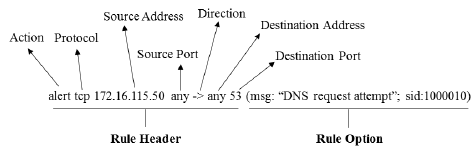
\includegraphics[width=0.8\textwidth]{resources/rule.png}
      \caption[Struktur \emph{rule} Snort NIDPS]{Struktur \emph{rule} Snort NIDPS \citep{khamphakdee2014}}
    \end{figure}

    Beberapa \emph{option} yang biasa digunakan dalam Snort \emph{Rule} diantaranya:
    \begin{enumerate} 
      \item \emph{sid}, ID \emph{rule}
      \item \emph{msg}, pesan kesalahan yang ditampilkan ke pengelola atau log
      \item \emph{flow}, arah aliran paket dari atau ke server
      \item \emph{flags}, flag TCP yang dicari
      \item \emph{content}, konten yang dicocokkan berupa teks
      \item \emph{reference}, acuan \emph{vulnerability} yang diduga
    \end{enumerate} 

% \section{Komputasi Paralel}

%   % \blindtext

%   \subsection{Hukum Amdahl dan Hukum Gustafson}

%     Secara optimal, speedup yang dicapai dengan paralelisasi akan tumbuh secara linier. Namun kenyataannya, paralesisasi terbatas dengan porsi sistem yang dapat diparalelkan. Sehingga, speedup maksimum yang akan dicapai hanya akan sebesar konstanta tertentu \citep{amdahl}. Hipotesis ini dikenal dengan Hukum Amdahl dengan persamaan

%     \begin{equation}
%       S_{latensi}(s) = \frac{1}{1 - p + \frac{p}{s}}
%     \end{equation} \\
%     dengan $Q$ adalah jumlah simpul dan $P$ adalah jumlah pola.

%     Hukum Amdahl hanya berlaku pada kasus dengan ukuran masalah yang tetap. Pada prakteknya, semakin besar kapasitas komputasi, ukuran masalah yang dipecahkan juga semakin besar dengan jumlah data yang juga besar, sehingga waktu yang dihabiskan pada porsi sistem yang dapat diparalelkan juga makin besar \citep{gustafson}. Berdasarkan fakta tersebut, Gustafson mengajukan perbaikan pada Hukum Amdahl

%     \begin{equation}
%       S_{latensi}(s) = 1 - p + sp
%     \end{equation} \\

%     Terlihat bahwa Hukum Gustafson membuat speedup maksimum menjadi lebih linier dan realistis.

%   \subsection{\emph{Multiprocessing} dan \emph{Multithreading}}

%     Proses adalah program yang sedang dieksekusi. Ketika proses dijalankan, dia memiliki beberapa status: baru, berjalan, menunggu, siap, dan berhenti. Tiap proses memiliki informasi mengenai alokasi memori, status proses, dan isi CPU register yang disebut dengan konteks \citep{os}. Ketika proses ini pertama dilanjutkan dari keadaan menunggu, maka CPU akan memuat konteks proses. Jika ada, proses lain yang akan berjalan, maka CPU akan mengganti konteks proses dengan konteks proses baru yang akan berjalan. Hal ini dikenal dengan \emph{context switching}.

%     Satu proses dapat memiliki banyak thread. Thread didefinisikan sebagai unit terkecil eksekusi dari CPU \citep{os}. Thread dikenal pula dengan proses ringan. Berbeda dengan proses, thread pada proses yang sama dapat berbagi memori yang sama. Penggunaan thread dapat memungkinkan operasi yang IO-bound dan CPU-bound dapat berjalan bersamaan.

%     Multiprocessing yaitu teknik untuk menggunakan proses yang berbeda untuk melakukan suatu pekerjaan. Sedangkan multithreading yaitu teknik yang memungkinkan satu unit pemroses (seperti CPU dan GPU) untuk mengeksekusi banyak thread secara konkuren. Keuntungan multithreading dibandingkan multiprocess adalah masing-masing thread akan berbagi resource dari unit komputasi, seperti memori, cache dan translation lookaside buffer (TLB). Selain itu, komunikasi antar thread juga bisa dilakukan dengan menggunakan memori bersama. 

%   \subsection{Sinkronisasi}

%     Multithreading memungkinkan kita untuk saling berbagi memori yang sama. Namun, ada kerugian dari adanya sharing resource ini. Task antar thread harus menjamin bahwa mereka tidak mengakses dan menimpa memori yang sama atau mereka akan mengakibatkan nilai memori menjadi tidak konsisten. Masalah ini dikenal dengan \emph{race condition}. Race condition terjadi ketika dua atau lebih thread memasuki wilayah yang seharusnya hanya boleh dimasuki satu thread yang disebut \emph{critical section}. 

%     Untuk menghindari terjadinya race condition kita dapat melakukan sinkronisasi proses. Ada beberapa metode sinkronisasi proses yang akan digunakan pada penelitian ini:

%     \begin{enumerate}

%     \item
%     Mutex lock \\
%     Mutex 

%     \item
%     Semaphore \\

%     \item
%     Barrier \\

%     \end{enumerate}

%  Ketika beberapa thread akan menggunakan critical section, maka flag akan dipasang untuk mencegah thread lain masuk dalam critical section tersebut. Ketika thread tersebut telah keluar dari critical section, flag akan dicabut kembali dan thread lain akan dapat masuk ke dalam critical section. 

%     Ada banyak jenis implementasi dari flag yang 
%Hal ini bisa diatasi dengan memasang lock pada resoure yang mungkin akan diakses bersama-sama. Lock dapat memandaatkan mutex lock, semaphore, atau dll.

% \section{Struktur Data Trie}

  %Struktur data \emph{trie} adalah struktur data yang digunakan untuk menyimpan himpunan dinamis dari beberapa string \citep{trie59}. Struktur data trie merupakan jenis dari struktur pohon yang memiliki jumlah simpul anak yang tidak tentu. 
  % Secara umum, \emph{trie} dapat menggambarkan dengan .  % 
  %Simpul akar \emph{trie} akan dimulai dari simpul kosong. Lalu bercabang ketika ada karakter yang berbeda. Sehingga pencarian string dalam kamus dapat dilakukan dengan menelusuri tiap simpul pada \emph{trie}. Trie dapat dimodelkan sebagai sebuah finite automata. Tiap simpul dapat dimodelkan sebagai status dan huruf atau substring dimodelkan sebagai fungsi transisi. Lalu, setiap simpul awal dan simpul akhir akan ditandai secara khusus. Ketika simpul akhir tercapai, berarti salah satu pola ditemukan.

  %\begin{figure}[htb]
  %    \centering
  %    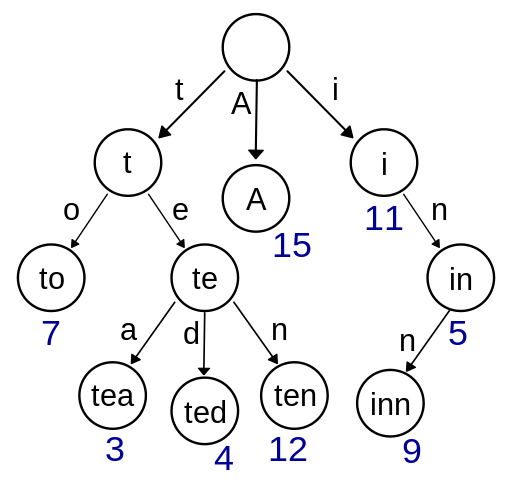
\includegraphics[width=0.8\textwidth]{resources/trie.png}
  %    \caption[Contoh trie untuk kata "A","to", "tea", "ted", "ten", "i", "in", dan "inn"]{Contoh trie untuk kata "A","to", "tea", "ted", "ten", "i", "in", dan "inn"}
  %  \end{figure}

  %Strategi implementasi yang biasa dilakukan yaitu dengan menggunakan list untuk menyimpan simpul anak sebanyak jumlah karakter maksimal pada tiap simpul. Bisa juga menggunakan tabel statik untuk menyimpan referensi ke simpul anak. 

  %\subsection{Bitwise Trie}

  %  Bitwise Trie adalah varian trie yang menggunakan operasi bit untuk penelusuran simpul. Berbeda dari trie yang menggunakan karakter sebagai fungsi transisi, bitwise trie hanya memiliki dua simpul anak tiap simpulnya. Meski terlihat lambat, metode ini mengoptimalkan cache lokal

  %\subsection{Trie dengan Kompresi}

\section{\emph{Pattern Matching}}

  \emph{Pattern matching} adalah metode mencari kemunculan sebuah string atau substring terhadap string lain. \emph{Pattern matching} menjadi salah satu komponen inti dalam NIDPS. Secara umum ada dua jenis utama pencocokan pola, yaitu \emph{single pattern matching} dan \emph{multi-pattern matching}. 
  
  \emph{Single pattern matching} yaitu pencocokan masukan terhadap satu pola. Algoritma yang tergolong \emph{single pattern matching} yaitu algoritma Knuth-Morris-Pratt dan Boyer-Moore. Sementara itu, \emph{multi-pattern matching} mencocokkan masukan terhadap beberapa pola sekaligus. Algoritma yang termasuk dalam \emph{multi-pattern matching} yaitu algoritma Aho-Corasick dan Wu-Manber, yang merupakan modifikasi dari algoritma Boyer-Moore. Fokus bahasan tugas akhir ini adalah \emph{multi-pattern matching}.

  \subsection{Algoritma Aho-Corasick}

    Algoritma Aho-Corasick adalah algoritma \emph{multi-pattern matching} yang dapat mencari kemunculan string dalam sebuah kamus \citep{ahoc1975}. Algoritma ini dapat mencari kemunculan setiap string dalam kamus dalam sekali pencocokan. Komponen utama dalam algoritma ini yaitu kamus yang berupa \emph{finite automata}. %dan \emph{failure transition}.

    Kamus berisi kumpulan string \emph{rule} yang akan dicocokkan. Penyusunan kamus hanya perlu dilakukan sekali sebelum pencocokan string dilakukan. Penyusunan kamus dilakukan dalam $O(kp)$, dengan $k$ adalah jumlah string pada kamus dan $p$ adalah panjang maksimum string pada kamus.

    Dalam kamus ada pula \emph{failure transition}. \emph{Failure transition} akan menunjuk ke posisi terakhir prefiks yang cocok dengan suffiks string yang dicari. Sehingga ketika pencarian tidak cocok pada suatu string, akan dilanjutkan pada string berikutnya yang prefiksnya cocok dengan suffiks string sebelumnya. Dengan \emph{failure transition}, pencocokan banyak pola dapat lebih efisien dibandingkan harus mengulang tiap pencarian dari awal. Kompleksitas pencarian algoritma ini yaitu $O(x)$, dengan $x$ adalah panjang string pola.

    \begin{figure}[htb]
      \centering
      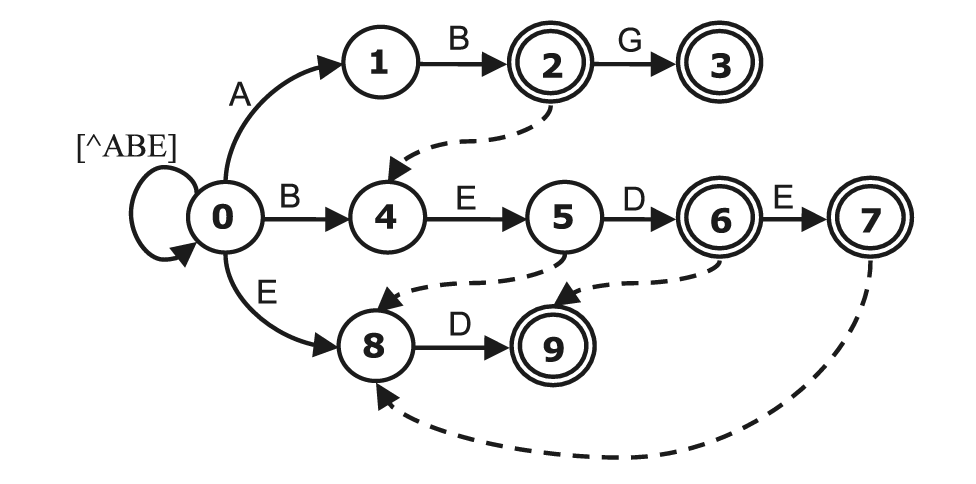
\includegraphics[width=0.6\textwidth]{resources/aho-c.png}
      \caption[\emph{Finite automata} kamus algoritma Aho-Corasick dengan \emph{failure transition}]{\emph{Finite automata} kamus algoritma Aho-Corasick dengan \emph{failure transition} \citep{lin2013}}
    \end{figure}

  \subsection {\emph{Boundary Detection Problem}}

    Untuk dapat meningkatkan kinerja algoritma Aho-Corasick, kamus dapat dipartisi menjadi beberapa segmen untuk tiap pola. Sehingga tiap partisi dapat digunakan untuk pencocokan pada tiap \emph{thread}. Namun terdapat ada masalah pada pencocokan partisi ketika pola yang dicari ternyata berada pada lebih dari satu partisi dan terpotong. Masalah ini dikenal sebagai \emph{boundary detection problem}. 

    \begin{figure}[htb]
      \centering
      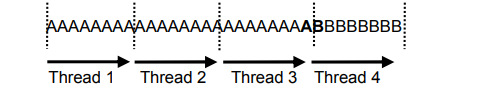
\includegraphics[width=0.5\textwidth]{resources/boundary.png}
      \caption[\emph{Boundary detection problem} terjadi pada pola "AB" tidak terbaca oleh \emph{thread} 3 dan 4]{\emph{Boundary detection problem} terjadi pada pola "AB" tidak terbaca oleh \emph{thread} 3 dan 4 \citep{lin2013}}
    \end{figure}

    Solusi dari masalah itu yaitu dengan menambah jangkauan pencocokan sepanjang $m - 1$, yaitu panjang pola terpanjang dikurangi satu. Total kompleksitas yang diperoleh tiap thread menjadi $O(n/s + m)$ dengan $n$ adalah panjang masukan dan $s$ adalah banyak segmen yang dibentuk. Sehingga total kompleksitas untuk lookup memori menjadi $O((n/s + m) * s) = O(n + ms)$. Dibandingkan dengan lookup pada Aho-Corasick standar yang hanya $(O(n)$, operasi ini bisa jadi akan menjadi bottleneck pada pencarian pola.

  \subsection {\emph{Parallel Failureless Aho-Corasick}}

    Algoritma \emph{Parallel Failureless Aho-Corasick} (PFAC) merupakan pengembangan dari algoritma Aho-Corasick untuk melakukan pencocokan dengan \emph{multithreading}. PFAC menggunakan \emph{state machine} yang tidak mengandung \emph{failure transition} dan masing-masing \emph{thread} memulai pencocokan dari tiap satu karakter masukan \citep{lin2013}.

    \begin{figure}[htb]
      \centering
      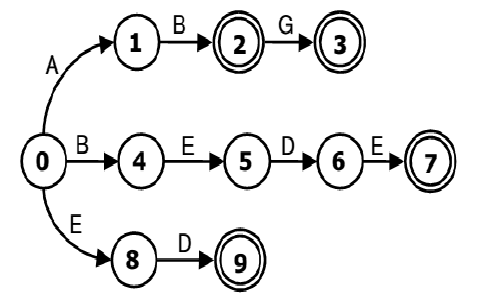
\includegraphics[width=0.5\textwidth]{resources/pfac.png}
      \caption[\emph{Finite automata} Aho-Corasick tanpa \emph{failure transition}]{\emph{Finite automata} Aho-Corasick tanpa \emph{failure transition} \citep{lin2013}}
    \end{figure}

\section{\emph{General-Purpose computing on Graphics Processing Units}}

  \emph{General-purpose computing on graphics processing units} (GPGPU, kadang disebut juga GPGP atau GP\textsuperscript{2}U) adalah teknik untuk menggunakan pemroses grafis / GPU untuk melakukan komputasi umum yang biasa dilakukan pada pemroses CPU. GPU memiliki banyak core yang berjalan paralel. Desain GPU berbeda dari CPU karena fokus GPU adalah melakukan operasi secara paralel. Berbeda dari CPU yang digunakan untuk melakukan operasi sekuensial \citep{lindholm2001}. Dalam GPU terdapat beberapa \emph{stream multiprocessor} (SM) yang masing-masing memiliki beberapa \emph{core thread} atau \emph{stream processor} (SP).

  \begin{figure}[htb]
    \centering
    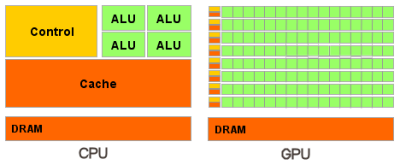
\includegraphics[width=0.8\textwidth]{resources/GPUvsCPU.png}
    \caption[Perbedaan arsitektur CPU dan GPU]{Perbedaan arsitektur CPU dan GPU \citep{cuda}}
  \end{figure}

  \subsection{Struktur Memori}
    
    Tiap \emph{core thread} memiliki memori lokal yang saling independen. Dalam tiap blok, \emph{thread} yang ada dalam blok dapat mengakses \emph{shared memory}. Kemudian ada memori global yang dapat diakses semua \emph{thread}. 
    
    Ada perbedaan kecepatan ketika melakukan operasi pada tiap tingkatan memori. Makin tinggi tingkatan memori, makin besar latensi akses memori. Urutan besar latensi akses memori yaitu memori lokal, memori bersama, kemudian memori global. Sehingga memori global tidak cocok digunakan untuk operasi yang tidak memerlukan sinkronisasi antar \emph{thread}. 
    
    Selain ketiga memori tersebut, ada juga memori yang hanya dapat ditulis oleh \emph{host} yaitu memori konstanta dan tekstur. Kedua memori ini hanya dapat ditulis sekali sebelum \emph{kernel} dipanggil. Keuntungan menggunakan kedua memori ini yaitu latensi akses yang lebih kecil dari memori global. Hal ini terjadi karena kedua memori ini memanfaatkan \emph{locality} dalam akses memori. Memori konstanta menggunakan \emph{cache} sehingga akses untuk memori yang sama berkali-kali akan sangat cepat. Sedangkan memory tekstur menggunakan \emph{spatial locality} untuk \emph{thread} yang berdekatan secara dua dimensi.

    \begin{figure}[htb]
      \centering
      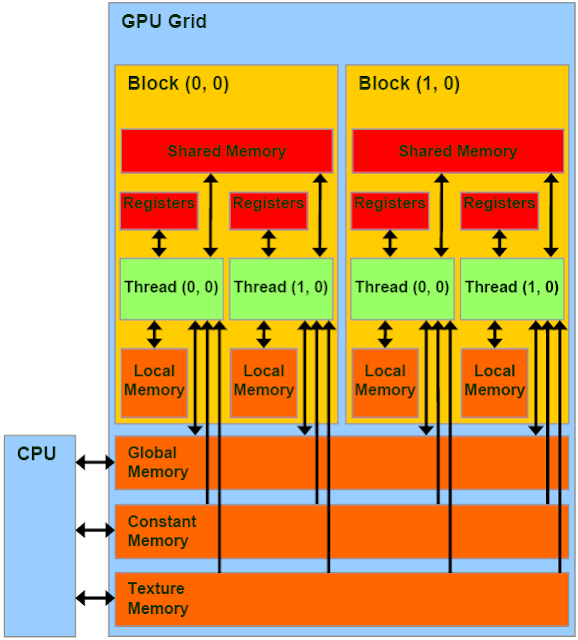
\includegraphics[width=0.8\textwidth]{resources/cudamem.png}
      \caption[Tingkatan memori GPU]{Tingkatan memori GPU \citep{cuda}}
    \end{figure}

  % Saat ini ada dua platform GPGPU yang populer, CUDA dan OpenCL. CUDA adalah platform yang dikembangkan oleh NVIDIA. CUDA hanya dapat berjalan pada perangkat milik NVIDIA. Sedangkan OpenCL dikembangkan oleh grup konsorsium Khronos. OpenCL dapat berjalan pada banyak perangkat, seperti CPU, GPU, FPGA, dan DSP (\emph{digital signal processor})).
  
  %Penelitian tentang GPGPU dimulai ketika \emph{programmable pixel} dan \emph{vertex shaders} diperkenalkan. Penggunaan GPGPU lebih mudah dengan adanya \emph{shading language} yang berjalan pada GPU. \emph{Shading language} adalah bahasa pemrograman yang spesifik untuk mendeskripsikan tampilan sebuah \emph{scene} \citep{proudfoot2001}. \emph{Shading language} bertujuan menyediakan antarmuka \emph{high level} untuk operasi \emph{vertex} pada GPU. 
  
  %Dengan adanya \emph{shading language}, operasi vektor dan matriks dapat dengan mudah diubah menjadi operasi \emph{vertex}. Sejak saat itu, usaha untuk melakukan komputasi umum dengan GPU mulai bermunculan seperti perkalian matriks \citep{matrix2001}, simulasi fisika \citep{phys2002}, hingga dekomposisi LU pada matriks persegi \citep{lugpu2005}. Maka, pada tahun 2003, dalam disertasinya \citep{harris2003}, Mark Harris mengajukan sebuah istilah yang kini dikenal sebagai \emph{general-purpose computing on graphics processing units} (GPGPU) sekaligus mendirikan situs GPGPU.org.
  
  \subsection{\emph{Compute Unified Device Architecture}}
  
    \emph{Compute Unified Device Architecture} (CUDA) adalah platform dan API untuk GPGPU oleh NVIDIA. CUDA menyediakan antarmuka untuk dapat menggunakan GPU NVIDIA untuk melakukan GPGPU \citep{cuda}. CUDA API dapat diimplementasi menggunakan bahasa C, C++, dan Fortran. Selain itu, ada juga \emph{binding} yang dibuat dalam pustaka beberapa bahasa oleh pihak ketiga, seperti Python, Perl, Java, Ruby, Haskell, Lua, MATLAB, dan Mathematica.
    
    \subsubsection{Struktur Kode CUDA}
    
      Terdapat dua perangkat yang berbeda untuk \emph{runtime} CUDA, yaitu \emph{host} (CPU), dan \emph{device} (GPU). Masing-masing platform akan menjalankan bagian kode tersendiri. Ada dua bagian dalam kode program CUDA, yaitu \emph{host code} dan \emph{kernel code}. Ketika program berjalan, maka \emph{host code} akan berjalan terlebih dahulu. Lalu, \emph{kernel code} akan disalin dan dijalankan di memori GPU. Karena memori yang dapat diakses oleh masing-masing kode juga terpisah, maka perlu dilakukan alokasi pada memori \emph{device} dan transfer antar memori \emph{device} dan memori \emph{host}.
    
    \subsubsection{\emph{CUDA Thread}}
    
      CUDA \emph{thread} dibagi menjadi beberapa kelompok blok yang disebut \emph{grid}. Masing-masing \emph{grid} berisi beberapa buah blok. Di dalam blok terdapat beberapa \emph{thread} yang akan berjalan terpisah. 
      
      \begin{figure}[htb]
        \centering
        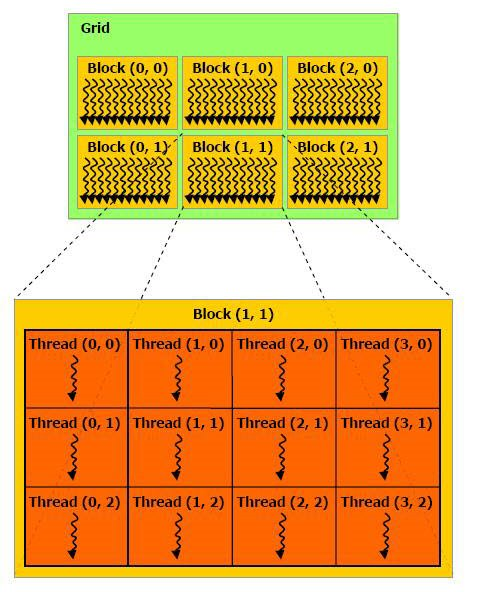
\includegraphics[width=0.8\textwidth]{resources/cudathread.jpg}
        \caption[Organisasi \emph{thread} CUDA]{Organisasi \emph{thread} CUDA \citep{cuda}}
      \end{figure}
      
      CUDA \emph{thread} memiliki indeks, yang berdimensi 3. Indeks \emph{thread} akan menunjukkan nomor blok dan nomor \emph{thread} tersebut dalam blok. Menggunakan kedua indeks tersebut, dapat dibentuk nomor yang unik tiap \emph{thread}. Nomor unik tersebut dapat digunakan untuk melakukan pemrosesan paralel pada data besar. Hingga CUDA versi 8.0, maksimum dimensi blok \emph{thread}, dimensi grid, dan jumlah \emph{thread} tiap blok berturut-turut adalah 1024 x 1024 x 64, 65535 x 65535 x 65535, dan 1024.

    \subsubsection{\emph{Warp} dan Percabangan}

      \emph{Thread} akan dieksekusi bersama-sama dalam sebuah kumpulan yang disebut \emph{warp}. \emph{Thread} yang berjalan dalam satu \emph{warp} akan mengeksekusi instruksi yang sama dalam satu waktu. Ketika ada percabangan dalam instruksi, maka \emph{warp} tersebut akan berpisah. Ukuran maksimal \emph{warp} saat ini yaitu 32 \emph{thread}.

      Karena percabangan mempengaruhi eksekusi \emph{warp}, maka penempatan kondisi harus dilakukan secara hati-hati. Jika percabangan tidak dilakukan dengan benar dan menyebabkan banyak \emph{thread} terpisah, maka akan banyak \emph{warp} yang akan terbuang karena hanya mengeksekusi sedikit \emph{thread}.
      
      Pada GPU arsitektur Fermi, terdapat fitur yang disebut \emph{memory coalescing}. \emph{Memory coalescing} terjadi ketika semua \emph{thread} pada \emph{warp} yang sama mengakses memori yang kontigu. Fitur ini memungkinkan akses memori yang kontigu tersebut dilakukan dalam sekali \emph{request}.

\section{Penelitian Terkait}

  \subsection{Rancangan \emph{Multithreading} pada Pencocokan NIDS Berbasis \emph{Signature}} 

    Penelitian terkait optimasi berbasis \emph{multithreading} pada NIDS telah dilakukan oleh \citep{multi2004}. Tujuan optimasi yaitu untuk meningkatkan kapasitas pencocokan signature. Optimasi dilakukan pada komponen-komponen berikut:

    \begin{enumerate}
      \item \emph{Thread} untuk modul keluaran yang terpisah
      \item Pencocokan signature secara \emph{multithread}
      \item Normalisasi konteks dan pencocokan signature secara \emph{multithread}
      \item Pencegahan \emph{stateful}, normalisasi konteks dan pencocokan signature secara \emph{multithread}
      \item Pencegahan \emph{stateful} secara \emph{multithread} dengan normalisasi konteks dan pencocokan signature secara \emph{multithread} terpisah
    \end{enumerate}

    Hasil yang diperoleh dengan pengukuran pada prosesor Intel Xeon dengan \emph{hyper-threading} menunjukkan bahwa desain 2 dan 3 memiliki kinerja yang rata-rata lebih baik dari pada desain lainnya. Pada desain 2 diperoleh penurunan runtime menjadi 94,1\% dan 86,1\%, untuk menggunakan \emph{hyper-threading enabled} dan tidak. Sedangkan pada desain 3, diperoleh runtime 89\% dan 84\%. Hal ini disebabkan \emph{latency} dari penggunaan \emph{shared memory} pada desain 4 dan 5 yang terlalu besar.

  \subsection{Rancangan NIDS berbasis GPGPU}

    Selain rancangan \emph{multithreading} pada CPU, telah dilakukan penelitian tentang rancangan arsitektur untuk NIDS pada GPGPU \citep{gnort2008}. Rancangan bertujuan mengakomodasi implementasi algoritma Aho-Corasick pada GPU. Beberapa komponen yang dimodifikasi yaitu implementasi \emph{state machine} dan skema transfer antara \emph{host} dan \emph{device}.

    Implementasi Snort menggunakan struktur memori untuk menyimpan pola \emph{signature} yang berbentuk \emph{list of string}. \emph{Layout} ini kemudian dimodfikasi menjadi \emph{array} 2D sebelum diimplementasi menggunakan CUDA. Kelebihan \emph{layout} memori ini adalah mudah untuk ditransfer ke memori tekstur. Selain itu algoritma Aho-Corasick memanfaatkan prinsip \emph{locality} dengan baik. Sehingga implementasi memori dapat meningkatkan kinerja pencocokan NIPS hingga 19\%.

    Transfer data dari \emph{host} ke \emph{device} maupun \emph{device} ke \emph{host} menggunakan skema \emph{double buffering}. Skema ini menggunakan sebuah \emph{buffer} untuk menampung paket yang ingin dicek menjadi satu batch besar. Batch besar kemudian ditransfer ke memori \emph{device}. Ketika GPU melakukan pemrosesan, maka paket yang baru datang akan ditampung dalam \emph{buffer} berbeda. Sehingga kedua \emph{buffer} dapat selalu bertukar posisi. Hal ini mampu meningkatkan utilitas pengiriman rata-rata paket. Selain itu, memori \emph{host} dapat dikonfigurasi menggunakan \emph{pinned memory} agar menurunkan tingkat \emph{memory page swapping} dan juga meningkatkan \emph{throughput} sistem.

    Ada 2 desain pencocokan paket yang diteliti:
    \begin{enumerate}

      \item Pencocokan paralel paket tunggal \\
      Paket akan dibagi menjadi fragmen-fragmen dan disebar merata pada tiap \emph{thread}. Kelebihan dari skema ini yaitu masing-masing \emph{thread} mendapat bagian yang setara dan waktu yang diperlukan untuk pencocokan relatif sama sehingga tidak perlu saling menunggu. Sedangkan kekurangan dari skema ini adalah pencocokan akan mengalami overlap satu sama lain dan perlu penanganan khusus.

      \item Pencocokan paralel multipaket \\
      Masing-masing paket akan didelegasikan pada satu \emph{thread} pada \emph{stream processor}. Kelebihan dari skema ini adalah pencocokan tidak akan mengalami overlap. Sedangkan kekurangan dari skema ini adalah pencocokan harus menunggu satu sama lain karena ukuran paket yang berbeda-beda.

    \end{enumerate}

    Berdasarkan pengujian yang menggunakan 1000 pola acak, pencocokan dengan GPU mendapat \emph{throughput} hingga 2,3 Gbps untuk paket 1500 \emph{byte}. Peningkatan yang berhasil dicapai sebesar 3,2 kali lipat. Spesifikasi lingkungan pengujian yaitu GPU NVIDIA GeForce 8600GT 1,2 GHz dengan 32 stream processor dalam 4 multiprocessor dan memori 512 MB, dan CPU Intel Pentium 4 3,4 Ghz dengan memori 2 GB.

  \subsection{Rancangan NIDS Berbasis \emph{Signature} yang \emph{Scalable} pada GPU}

    Dalam penelitiannya, dijelaskan oleh \citep{kargus2012} bahwa pada NIDPS, \emph{bottleneck} utama terdapat pada 3 komponen, \emph{packet acquisition}, \emph{multi-string pattern matching}, dan pencocokan opsi \emph{rule}. Pencocokan opsi \emph{rule} hanya dilakukan saat paket terindikasi mengandung serangan oleh tahap multi-string pattern matching. Sebelum PCRE dicocokkan, PCRE akan dipreproses menjadi DFA terlebih dahulu menggunakan algoritma Thompson. Kemudian pencocokan opsi dapat dilakukan menggunakan metode yang serupa dengan pencocokan \emph{multi-string}.

    Salah satu optimasi yang diajukan untuk tahap pencocokan yaitu penggunaan \emph{pipelining}. \emph{Pipelining} dilakukan dengan memisahkan \emph{thread} yang digunakan untuk operasi \emph{I/O} dengan operasi analisis. Kemudian pada tiap operasi \emph{I/O}, akan dilakukan pengumpulan paket dalam \emph{batch} sebelum dilakukan transfer antar komponen. 

    Pengujian dilakukan dengan konfigurasi CPU ganda Intel X5680 dengan 12 core dan dua GPU NVIDIA GTX580. Hasil yang didapatkan menggunakan desain ini mampu mencapai 1,5 sampai 4 kali lipat kinerja Snort. \emph{Latency} dapat menurun hingga 13 mikrodetik pada \emph{offloading} paket awal untuk batch sebesar 1,5 kB. Pada pengujian dengan \emph{traffic} jaringan, rancangan ini mampu mencapai \emph{throughput} 25,2 Gbps pada \emph{input} sebesar 40 Gbps.

  \subsection{Penyimpanan \emph{Signature} dengan Struktur \emph{Trie} Terkompresi}

    Penyimpanan \emph{signature} untuk NIDS dapat dilakukan dengan struktur \emph{trie} terkompresi \citep{bellekens2014}. Desain utama \emph{trie} menggunakan representasi penelusuran \emph{breadth first search} (BFS). Lokasi \emph{pointer} simpul anak akan dihitung menggunakan \emph{sparse matrix}. Selain itu dilakukan kompresi terhadap bentuk \emph{trie} sehingga memori yang dibutuhkan lebih padat.

    Masing-masing simpul dalam \emph{trie} akan mengandung tiga buah informasi, matriks akan berisi \emph{offset} dari lokasi simpul anak terkecil dan sebuah \emph{bitmap} berisi flag dari semua simpul anak dalam 256 karakter ASCII. Ketika ingin melakukan penelusuran, simpul akan melakukan penghitungan karakter berdasarkan offset pertama simpul ditambah dengan kumulatif dari tiap bit.

    Optimasi berikutnya yaitu kompresi pada suffiks kalimat. Kompresi dilakukan dalam dua tahap: penggabungan pada huruf terakhir dan tiga huruf terakhir yang sama. Huruf terakhir dapat digabungkan karena simpul tersebut tidak memiliki anak lagi. Dan tiap simpul tersebut pasti akan menuju ke penanda akhir string. Jumlah simpul dapat dihitung ulang dengan persamaan berikut: \\
    \begin{equation}
      Q_{final} = Q - \left(\left|P\right| - 1 \right)
    \end{equation} \\
    dengan $Q$ adalah jumlah simpul dan $P$ adalah jumlah pola.

    Kemudian untuk tahap kedua, akan dihitung suffiks dari pola. Tiap suffiks tiga karakter terakhir yang sama akan digabungkan. Jumlah kombinasi dari susunan dua karakter dapat dihitung dengan \\
    \begin{equation}
      r = S^2
    \end{equation} \\
    dengan $r$ adalah jumlah kombinasi susunan dan $S$ adalah banyak huruf yang ada dalam string pola.

    Maka, jumlah kombinasi dari \emph{trie} dapat diestimasi dengan \\
    \begin{equation}
      \overline{L} = 
        \sum_{i=1}^{r} P\left(g = i \right) \cdot 2i =
          \sum_{i=1}^{min\left({r,n} \right)} \frac{\binom{r}{i} \binom{n - i}{i}}{\binom{n}{r}} \cdot 2i
    \end{equation} \\
    dengan $L$ adalah rata-rata panjang \emph{trie} setelah kompresi, $P$ adalah kemungkinan \emph{trie} memiliki suffiks unik sejumlah $i$.

    %!TeX root=../thesis.tex

\chapter{Analisis Permasalahan dan Solusi}

  % Pada bab ini akan dipaparkan analisis berdasarkan studi literatur pada bab sebelumnya terkait pembangunan sistem pencegahan intrusi berbasis GPU. Selain itu, akan dipaparkan juga solusi yang diajukan untuk mesin yang akan dibuat.

  \section{Analisis Permasalahan}
  
    % Sistem pencegah intrusi jaringan (NIPS) adalah sistem yang bertugas melakukan penyaringan paket yang dianggap berbahaya. NIPS bekerja dengan cara menangkap paket yang berjalan dalam jaringan untuk kemudian dianalisis. Hasil analisis kemudian ditindaklanjuti berdasarkan \emph{rule} yang telah didefinisikan. Paket dapat ditolak, dibatasi atau bahkan diblok.

    % Analisis paket dapat dilakukan dengan bermacam-macam metode asd

    Dampak dari pengecekan paket adalah adanya \emph{overhead} waktu respons. Lama \emph{overhead} tergantung dari waktu pencocokan pola. Pada sistem pencegah intrusi jaringan (NIPS), hal ini dapat membuat hasil analisis menjadi tidak akurat. Maka perlu adanya metode untuk mempercepat proses analisis. Sebagai perbandingan, \emph{bandwidth} jaringan US Naval Postgraduate School sudah mencapai 20 Gbps dengan traffic rata-rata sebesar 200 Mbps per hari. Sedangkan maksimum paket yang dapat dianalisis secara serial oleh Snort tidak lebih besar dari 300 Mbps \citep{albin2012}.

    Beberapa penelitian tentang teknik mempercepat NIDS dan NIPS telah dilakukan. Desain paling awal yaitu menggunakan desain konkuren dengan \emph{multithreading} pada CPU \citep{multi2004}. Desain ini mampu meningkatkan penggunaan utilitas \emph{thread} CPU secara drastis. Kemudian desain berbeda yang menggunakan GPU mulai diajukan oleh \cite{gnort2008}. Hasil yang didapat mampu mempercepat sistem hingga 5x dibandingkan CPU dengan harga yang sepadan \citep{smith2009}.

    % Pencocokan dapat dilakukan secara stateful, ataupun tidak. Pencocokan yang berbasis stateful akan lebih susah untuk dicek secara paralel.

    %Meski demikian, masih ada beberapa masalah terjadi dalam desain yang telah diajukan. Pencocokan paket masih menggunakan algoritma yang berbasis backtracking sehingga banyak operasi sinkronisasi yang menghambat laju pencocokan dengan multithread.  Selain itu, opsi pada rule seringkali tidak dapat dicocokkan dengan sekali asd

    Berdasarkan pengukuran yang dilakukan oleh \cite{kargus2012}, didapatkan bahwa sebagian besar beban analisa paket berada pada tahap pencarian string pada \emph{payload} paket. Pada tahapan ini, sebagian besar paket yang tidak terindikasi sebagai serangan akan diloloskan. Sehingga beban pencocokan pada tahap berikutnya, yaitu pencocokan \emph{option rule} akan berkurang drastis. Maka, fokus dari solusi yang akan diajukan yaitu implementasi desain yang akan mempercepat kinerja pencocokan string paket pada NIDS Snort.

  \section{Analisis Solusi}

    Eksperimen penggunaan GPGPU pada NIDS akan memodifikasi NIDPS Snort. Snort digunakan karena kode bersifat \emph{open-source} dan mudah untuk dikembangkan, sehingga pengembangan dan eksperimen tidak memerlukan banyak biaya dan dapat dieksplorasi secara mandiri. 

    Pengembangan akan menggunakan platform GPGPU CUDA. Platform CUDA merupakan platform GPGPU yang dibuat pada GPU NVIDIA. Platform CUDA digunakan karena saat ini platform CUDA lebih matang daripada OpenCL. Selain itu, dokumentasi dan contoh CUDA lebih banyak dan API yang lebih sederhana dan spesifik dibanding OpenCL.

    \subsection{Struktur IDS Snort}

      Komponen utama yang akan dioptimasi yaitu pencocokan string yang dilakukan setelah preproses. Pencocokan string dilakukan pada modul MPSE (\emph{multipattern search engine}). Modul ini dipanggil ketika \emph{rule} selesai dikelompokkan berdasarkan servis dan protokol seperti terlihat pada Gambar III.1 di bawah. Tiap \emph{rule group} akan memiliki \emph{instance} MPSE sendiri dan membentuk kamus sesuai \emph{rule} yang ada pada tiap \emph{rule group}.

      \begin{figure}[htb]
        \centering
        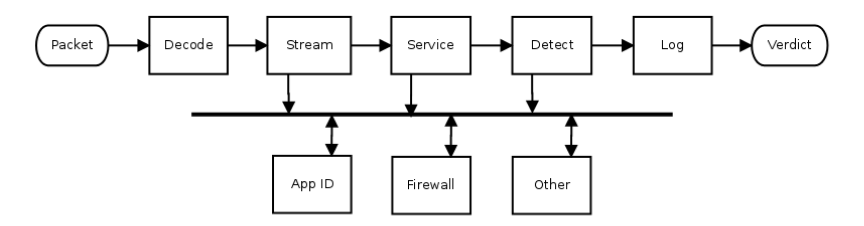
\includegraphics[width=0.8\textwidth]{resources/snort3.png}
        \caption[Arsitektur Snort versi 3]{Arsitektur Snort versi 3. Pencocokan dilakukan pada bagian Detect}
      \end{figure}

      Setelah pembentukan \emph{instance} dilakukan, maka input akan di-\emph{streaming}, dipreproses, dibagi berdasarkan \emph{rule group}, kemudian disuplai ke \emph{instance} MPSE yang terkait. Hasil pencocokan paket akan dikumpulkan dalam \emph{reducer} untuk kemudian dibandingkan dengan \emph{policy} apakah dianggap paket berbahaya atau tidak.

    \subsection{Algoritma Pencocokan \emph{Signature}}

      Komponen utama yang akan dioptimasi yaitu pencocokan string. Diantara pencocokan pola yang digunakan pada Snort, versi Aho-Corasick memiliki runtime yang paling cepat menggunakan teknik \emph{multithreading} pada CPU. Idealnya, modul yang ingin dikembangkan akan melampaui kinerja dari Snort yang menggunakan algoritma Aho-Corasick ini.
      
      Berdasarkan pengujian eksperimen yang dilakukan oleh \cite{lin2013}, implementasi langsung dari algoritma ini tidak memiliki keunggulan yang signifikan pada GPU. Salah satu kendala dari algoritma AC (Aho-Corasick) adalah \emph{boundary matching problem}. Masalah ini bisa diatasi dengan menambahkan jangkauan pencarian sebesar pola terpanjang. Namun, efek dari trik ini adalah peningkatan kompleksitas yang cukup drastis dari $O(n)$ menjadi $O(n + ms)$. 
      
      Solusi yang diajukan oleh \cite{lin2013} yaitu dengan menggunakan algoritma PFAC (\emph{Paralel Failureless Aho-Corasick}). PFAC adalah varian dari AC yang memulai pencocokan \emph{thread} pada tiap karakter dan tidak menggunakan \emph{failure transition}. Ada beberapa keuntungan dari algoritma ini:
    
      \begin{enumerate}

        \item 
        Tiap \emph{thread} hanya bertanggung jawab dengan string yang dimulai dengan karakter pada \emph{thread} tersebut. Ketika tidak ada pola yang cocok dengan huruf pada \emph{thread}, pencarian langsung berhenti pada \emph{thread}. Akibatnya, umur \emph{thread} juga lebih singkat.
        
        \item 
        Dalam mesin PFAC, tiap 32 \emph{thread} dalam \emph{warp} akan mengakses memori yang berurutan dari memori global. Dengan demikian, akses tabel transisi fitur \emph{memory coalescing} dapat dimanfaatkan.
        
        \item
        Tidak memerlukan penyimpanan tambahan untuk \emph{failure transition}. Sehingga konsumsi memori akan lebih sedikit dan kemungkinan \emph{cache hit} lebih besar.
        
      \end{enumerate}
      
      % \subsection{Skema Pengiriman Paket ke GPU}
      
      %  Operasi yang cukup sering akan dilakukan dalam Snort NIPS adalah pengiriman paket dari stream 
      %  Salah satu komponen yang paling penting dalam GPGPU adalah penyalinan data antar host dan device. Pengiriman dari host ke device maupun sebaliknya memiliki \emph{latency} yang cukup besar. Dalam pengujian pada \citep{gnort2008}, didapatkan bahwa \emph{latency} dari transfer payload memiliki runtime lebih dari 80\% runtime total. Sehingga untuk menyembunyikan \emph{latency}, pengujian akan menggunakan batch processing.      
      % pengiriman akan dilakukan per batch. Ukuran batch yang digunakan akan diuji dalam ukuran 32MB, 64MB, 128MB, dan 256MB.
      
      \subsection{Struktur Penyimpanan Kamus}
      
      Implementasi dari mesin PFAC yang digunakan ada beberapa macam. Salah satu model yang dapat digunakan yaitu dengan bentuk seperti pohon dengan \emph{list of pointer} ke status anak. Namun, model yang dialokasi secara dinamis tidak cocok digunakan dalam GPU karena alokasi pada GPU memiliki latensi yang tinggi. Selain itu, lokasi memori dapat menjadi tidak kontigu dan tidak mendukung adanya \emph{spatial locality}.
      
      Opsi lainnya yaitu dengan tabel transisi dua dimensi. Untuk tiap status, akan dibuat daftar status transisi terhadap tiap karakter. Model ini lebih sederhana dan juga mendukung adanya \emph{memory coalescing}. Tabel akan dibentuk di \emph{host memory}. Setelah semua pola didaftarkan, tabel akan disalin ke GPU hanya sebesar ukuran tabel yang terisi agar tidak boros memori. Tiap baris menunjukkan transisi dari tiap status yang bukan status akhir dan memiliki 256 kolom. Tabel transisi akan berbentuk seperti Gambar III.2 di bawah.

      \begin{figure}[htb]
        \centering
        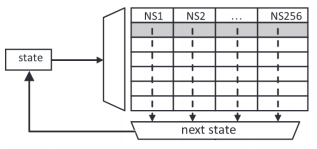
\includegraphics[width=0.6\textwidth]{resources/table.png}
        \caption[Tabel transisi]{Tabel transisi dari \emph{state machine} kamus}
      \end{figure}

      Untuk mengurangi kebutuhan terhadap penanda status akhir, nomor status akan disusun ulang. Status akhir akan diletakkan pada status pertama hingga ke-N. Sedangkan status lainnya termasuk status awal dimulai dari N+1. Dengan demikian, kebutuhan memori untuk penanda akan berkurang. Selain itu, operasi pengecekan dalam kode \emph{kernel} lebih sederhana dan ringan.

      Penghematan memori lebih jauh dapat dilakukan dengan menerapkan skema kompresi tabel menjadi \emph{bitmap}. Namun, keuntungan dari penggunaan memori tekstur akan terhambat. Dibutuhkan komputasi tambahan untuk melakukan \emph{lookup fetch} dari memori tekstur. Sehingga teknik ini tidak digunakan pada rancangan modul.

      \subsection{Alokasi \emph{Thread}}

      Seperti dijelaskan pada bagian III.2.1, \emph{thread} akan menelusuri \emph{state machine} yang sama dan berhenti ketika tidak ada transisi yang valid. Sehingga, banyak diantara \emph{thread} yang akan berhenti sangat awal. Untuk menunjang \emph{stream processor}, \cite{lin2013} mengusulkan alokasi memori yang berulang.

      Dalam satu blok, satu atau beberapa \emph{byte stream} akan ditempatkan sebagai lokasi awal satu \emph{thread}. Misal, dalam blok berisi 4.096 \emph{byte} dengan 512 \emph{thread}, \emph{thread} pertama akan memulai pencocokan pada posisi kelipatan 512. 

      Akibat dari penugasan yang berulang, diharapkan kemungkinan ketimpangan muatan dari masing-masing \emph{thread} akan berkurang. Pengujian yang dilakukan oleh \cite{lin2013} menunjukkan hasil serupa. Sehingga, skema inilah yang akan digunakan dalam implementasi kode \emph{kernel}. %Kode \emph{kernel} akan menerima \emph{stream} sebesar 128 kB dengan 512 \emph{thread}.
      
      % Penyimpanan \emph{signature} mempengaruhi besar memori yang digunakan. Struktur yang digunakan akan menggunakan trie terkompresi. Struktur digunakan untuk memaksimalkan \emph{locality} sehingga mengurangi \emph{latency}. Selain itu, dengan menurunkan konsumsi memori, besar buffer yang dapat digunakan meningkat. Diharapkan, \emph{latency} dari pengiriman juga menurun.
      
      % Penggunaan texture memory diharapkan dapat membantu menurunkan latency dalam pembacaan tabel.
      
      \subsection{Optimasi Latensi pada GPU}
      
      Pencocokan pola dengan tabel transisi adalah aplikasi yang \emph{memory-bound}. Penyimpanan pola pada memori global adalah salah satu sumber latensi. Salah satu optimasi yang dapat digunakan yaitu menyimpan pola pada memori tekstur. Memori tesktur dapat digunakan untuk mengurangi latensi pada \emph{state} yang berdekatan atau sering diakses. Berdasarkan \cite{lin2013}, penggunaan memori tekstur dapat menurunkan latensi hingga 12\%. Lebih lanjut, dapat dilakukan pemuatan baris pertama tabel transisi, yaitu baris milik status awal, ke dalam \emph{shared memory} karena baris ini yang pasti akan digunakan semua \emph{thread}. Peningkatan dari memuat baris pertama ke \emph{shared memory} akan berdampak besar ke latensi sistem.
      
      % Memori konstanta unggul ketika pola yang dicocokkan sedikit bercabang. Jika pola yang dicocokkan sedikit bercabang, maka \emph{cache} dapat dimanfaatkan dan latensi berkurang secara signifikan. Namun, pada ruleset Talos, tidak banyak rule yang sama sehingga juga akan banyak terjadi \emph{cache miss}. Akibatnya memori konstanta tidak lagi unggul. 
      
      Kemudian sumber latensi kedua adalah mengambil karakter dari \emph{stream} masukan. Ketika pencocokan dilakukan, \emph{thread} yang bersebelahan akan mengakses karakter dalam \emph{stream input} yang sebelumnya diakses oleh \emph{thread} lain. Berdasarkan skenario ini, \cite{lin2013} mengusulkan untuk menyalin string masukan ke \emph{shared memory} terlebih dahulu. Selain itu untuk mencegah masukan pada memori global terkena \emph{swap}, maka \emph{stream buffer} akan menggunakan \emph{pinned memory}. 

  \section{Rancangan Solusi}

    Pembahasan mengenai rancangan solusi dibagi menjadi 3 bagian. Bagian pertama dibahas mengenai gambaran umum solusi. Bagian kedua dibahas mengenai kebutuhan perangkat lunak. Bagian ketiga dibahas arsitektur perangkat lunak. 

    \subsection{Gambaran Umum Solusi}

      Berdasarkan analisis yang telah dilakukan, NIDS akan dikembangkan dari NIDS Snort dengan beberapa metode. Metode pengembangan akan mengacu pada implementasi \cite{lin2013} serta sedikit penyesuaian untuk berdasarkan \cite{gnort2008}.
      
      % Algoritma pencocokan yang akan digunakan adalah PFAC. Tabel transisi akan menggunakan tabel dua dimensi dengan jumlah kolom sebesar ukuran karakter, yaitu 256 \emph{byte}. Kemudian tabel ini akan diikat ke memori tekstur. Sedangkan \emph{buffer payload} akan menggunakan metode \emph{batching} dengan \emph{pinned memory}.

      Secara garis besar, terdapat 4 tahapan yang harus dilakukan dalam modul pencocokan pola yang akan dibangun:

      \begin{enumerate}

      \item
      Pembentukan tabel transisi \\
      Pembentukan tabel transisi akan dilakukan saat persiapan pencocokan. Struktur
      tabel dan operasi pembentukan didasarkan pada \cite{lin2013}. Struktur akan
      menggunakan tabel transisi 2D dengan struktur internal larik 1D. Pembentukan dilakukan pada \emph{host} kemudian baru akan ditransfer ke \emph{device}. Pembentukan tabel transisi dilakukan dengan mengumpulkan pola terlebih dahulu. Setelah pola terkumpul, lalu \emph{state} akan disusun kembali agar \emph{state} akhir berada di bagian paling awal tabel. Sehingga \emph{state} selain \emph{state} akhir dimulai dari N+1 dengan N adalah jumlah pola. 

      \item
      Persiapan tabel transisi dalam \emph{device memory} \\
      Setelah tabel transisi dibentuk, tabel akan dikirimkan ke \emph{device memory}. Penyimpanan pola akan diikat pada memori tekstur sesuai \cite{lin2013}. Selain itu juga disiapkan tabel untuk menampung hasil pencocokan. Tabel akan dialokasikan sebesar jumlah \emph{thread} yang digunakan dalam pencocokan.

      \item
      Penampungan \emph{stream} masukan \\
      \emph{Stream} input akan ditampung dalam \emph{secondary buffer} hingga sebesar 256 kB. \emph{Buffer} akan dialokasi dengan \emph{pinned memory} untuk memungkinkan DMA (\emph{direct memory access}) dari memori \emph{host} ke \emph{device} \citep{gnort2008}. Kemudian setelah \emph{buffer} mendekati penuh, \emph{stream} akan ditransfer ke memori \emph{device}.

      \item
      Penelusuran automata \\
      Pencocokan dilakukan dengan penelusuran mesin PFAC yang sudah dibentuk. \emph{Stream} masukan akan dimuat pada \emph{shared memory}. Tiap \emph{thread} akan memulai pencocokan pada satu karakter pada \emph{stream} masukan. Satu \emph{thread} melakukan pencocokan sebanyak 4 kali untuk mengurangi kemungkinan ketimpangan beban \citep{lin2013}. Penelusuran dilakukan hingga mencapai state akhir. Jika state akhir bukan merupakan state dummy, maka hasil pencocokan akan diset pada tabel hasil yang berada di \emph{global memory}.

      \end{enumerate}

    \subsection{Kebutuhan Perangkat Lunak}

      Berdasarkan analisis yang dilakukan sebelumnya, NIDS yang akan dibangun setidaknya memiliki spesifikasi kebutuhan fungsional seperti yang dijabarkan dalam Tabel III.1.
      
      \begin {table}[h]
\begin{center}
\caption {Kebutuhan Fungsional}
\begin{tabular}{|p{.5cm}|l|}

\hline
\rowcolor{gray!10}
No & Kebutuhan Fungsional \\
\hline

1 & Mampu membaca paket dari berkas PCAP \\
\hline

2 & Mampu membuat struktur automata untuk pencocokan paket \\
\hline

3 & Mampu menjalankan pencocokan pada GPU \\
\hline

4 & Mampu menghasilkan \emph{alert} pada paket yang terindikasi berbahaya \\
\hline

\end{tabular}
\end{center}
\end{table}


      % Berdasarkan Kebutuhan fungsional tersebut maka diagram \emph{use case} dari NIDS yang akan dibangun adalah seperti pada Gambar III.1 berikut

      % \begin{figure}[htb]
  \centering
  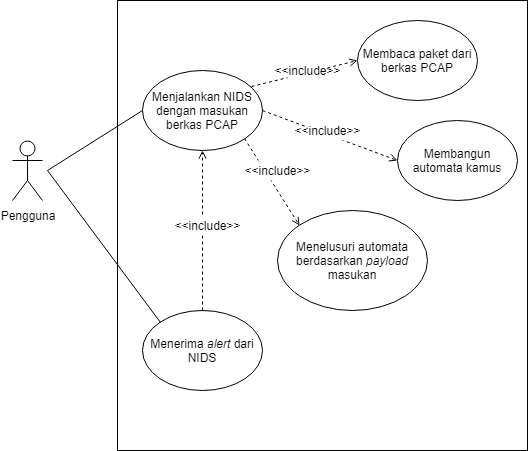
\includegraphics[width=1.0\textwidth]{resources/use-case.png}
  \caption[Diagram \emph{Use Case}]{Diagram \emph{Use Case}}
\end{figure}

    \subsection{Arsitektur Perangkat Lunak}

      Arsitektur yang digunakan akan menggunakan arsitektur dasar Snort. Dalam mengimplementasikan modul pencocokan, Snort menyediakan API yang dapat diimplementasi dengan mudah. Sehingga dalam penggabungan modul tersebut, hanya perlu dibuat \emph{wrapper} untuk memanggil modul yang telah diimplementasi secara terpisah.

      Modul akan terdiri dari beberapa komponen. Komponen-komponen tersebut akan tersusun menjadi sebuah \emph{pipeline} seperti pada Gambar III.1. Ada beberapa komponen utama dalam modul pencocokan pola:

      \begin{figure}[htb]
  \centering
  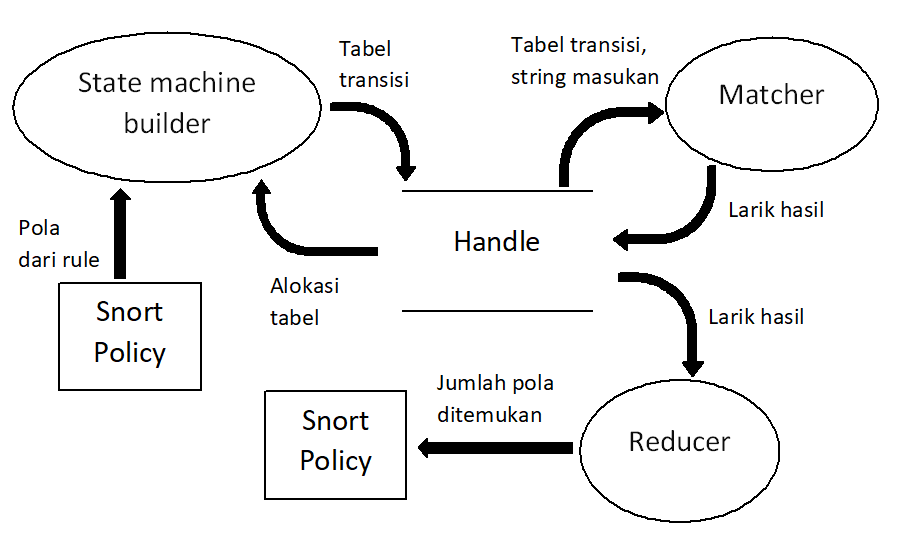
\includegraphics[width=0.5\textwidth]{resources/module-arch.png}
  \caption[Arsitektur modul]{Arsitektur modul}
\end{figure}
      
      \begin{enumerate}

        \item 
        \emph{Pattern builder} \\
        \emph{Pattern builder} melakukan pembangkitan kamus dari \emph{ruleset}. Pola akan ditambahkan dalam bentuk \emph{list of string} untuk kemudian ditampung dalam \emph{temporary table}. Kemudian \emph{temporary table} akan diiterasi untuk membentuk kamus. Kamus yang dibentuk menggunakan struktur tabel 2D dengan baris sebagai \emph{state} dan kolom sebagai status transisi. Setiap baris memiliki kolom sebesar 256 \emph{byte}.

        \item
        \emph{Matcher} \\
        \emph{Matcher} akan menyalin \emph{stream} dari \emph{host buffer} ke \emph{device buffer}. Kemudian \emph{stream} dari \emph{buffer} akan disalin ke \emph{shared memory}. Setelah \emph{stream} siap, \emph{matcher} akan melakukan pencocokan dengan menelusuri kamus secara paralel berdasarkan tiap karakter.

        \item
        \emph{Reducer} \\
        \emph{Reducer} akan menggabungkan hasil pencocokan dari tiap \emph{byte} sehingga diperoleh jumlah total rule yang terdeteksi. Jumlah ini akan dibandingkan dengan \emph{policy} oleh Snort untuk menentukan apakah \emph{stream} dianggap berbahaya atau tidak. \emph{Reducing} akan dilakukan secara sekuensial pada CPU.
        
      \end{enumerate}
    %!TeX root=../thesis.tex

\chapter{Implementasi dan Pengujian}

Pembahasan pada bab ini akan dibagi menjadi dua bagian. Bagian pertama dipaparkan tentang lingkungan dan detail implementasi. Sedangkan bagian kedua dibahas mengenai teknis dan hasil pengujian terhadap perangkat lunak yang sudah dibangun.

\section{Implementasi}

  Bagian implementasi dibagi menjadi 4 bagian. Bagian pertama dibahas mengenai lingkungan implementasi. Bagian kedua dibahas mengenai batasan implementasi. Bagian ketiga dibahas mengenai spesifikasi modul. Bagian terakhir berisi konfigurasi sistem deteksi intrusi.

  \subsection{Lingkungan Implementasi}

    Dalam proses implementasi digunakan sebuah laptop dan sejumlah perangkat lunak untuk menyelesaikan perangkat lunak yang dibangun. Detil spesifikasi perangkat keras dan lunak yang digunakan adalah seperti pada Tabel IV.1.
    
    \begin {table}[h]
\begin{center}
\caption {Spesifikasi Lingkungan Implementasi}
\begin{tabular}{|l|l|}

\hline
\rowcolor{gray!10}
Komponen & Spesifikasi \\
\hline

Sistem Operasi & Ubuntu 16.04.2 AMD 64-bit \\
\hline

CPU & Intel{\textregistered} Core{\texttrademark} i7-7500U CPU @ 2.70GHz × 4 \\
\hline

Host RAM & 16 GB \\
\hline

GPU & NVidia GeForce 940MX Compute Capablity 4.0 \\
\hline

Media Penyimpanan & \emph{Solid state drive} Samsung EVO 850 1TB \\
\hline

Dedicated Video RAM & 2 GB \\
\hline

CUDA Runtime & CUDA 8.0 r2 \\
\hline

G++ Compiler & GCC ??? \\
\hline

\end{tabular}
\end{center}
\end{table}


  \subsection{Batasan Implementasi}

    Implementasi dilakukan dengan batasan-batasan sebagai berikut.

    \begin{enumerate}

      \item
      Pencocokan menggunakan satu instance GPU \\
    
      \item
      Pencocokan hanya dilakukan satu kernel code \\
    
      \item
      Masukan paket hanya dilakukan dari berkas PCAP \\
    
%    \item
%    Konfigurasi dilakuakn

    \end{enumerate}

  \subsection{Spesifikasi Modul}
  
   \begin{enumerate}

      \item
      Komponen pembentukan kamus \\
    
      \item
      Komponen pencocokan \\
    
      \item
      Komponen penggabungan hasil \\

    \end{enumerate}

  \subsection{Konfigurasi}
    \blindtext

\section{Pengujian}

  \subsection{Tujuan Pengujian}
    Pengujian dilakukan untuk mendapatkan perbandingan kinerja antara modul yand dikembangkan dan modul yang ada dalam NIDS Snort. 

  \subsection{Skenario Pengujian}
  
    Pengujian dilakukan dengan membuat dua mesin, satu sebagai 
    Pengujian dilakukan dengan menerima masukan berupa berkas PCAP. Berkas didapatkan dari log traffic DEFCON ?? yang berlangsung pada ???. Dataset didapatkan dari ???.
    
  \subsection{Lingkungan Pengujian}
    
    Pengujian dilakukan pada mesin yang sama dengan lingkungan pengembangan.
    
    \begin {table}[h]
\begin{center}
\caption {Spesifikasi Lingkungan Implementasi}
\begin{tabular}{|l|l|}

\hline
\rowcolor{gray!10}
Komponen & Spesifikasi \\
\hline

Sistem Operasi & Ubuntu 16.04.2 AMD 64-bit \\
\hline

CPU & Intel{\textregistered} Core{\texttrademark} i7-7500U CPU @ 2.70GHz × 4 \\
\hline

Host RAM & 16 GB \\
\hline

GPU & NVidia GeForce 940MX Compute Capablity 4.0 \\
\hline

Media Penyimpanan & \emph{Solid state drive} Samsung EVO 850 1TB \\
\hline

Dedicated Video RAM & 2 GB \\
\hline

CUDA Runtime & CUDA 8.0 r2 \\
\hline

G++ Compiler & GCC ??? \\
\hline

\end{tabular}
\end{center}
\end{table}


  \subsection{Hasil Pengujian}
    \blindtext

  \subsection{Pembahasan}
    \blindtext
    \chapter{Simpulan dan Saran}

\section{Simpulan}
    Beberapa kesimpulan yang didapat dari pengerjaan tugas akhir ini adalah sebagai berikut.

    \begin{enumerate}

        \item 
        Peningkatan kinerja pencocokan string pada IDS Snort menggunakan GPU berhasil dilakukan dengan cara mengubah pendekatan algoritma yang digunakan agar memaksimalkan utilisasi GPU\%.

        \item
        Implementasi dilakukan dengan berbasis pada rancangan \cite{lin2013}, yaitu dengan Aho-Corasick varian tanpa \emph{failure function} dan delegasi \emph{thread} per karakter. Teknik ini memanfaatkan kemampuan GPU untuk membangkitakan banyak \emph{thread} serta \emph{memory coalescing} ketika mengakses karakter yang bersebelahan dalam \emph{stream}.
        
        \item 
        Operasi pencocokan string dari kamus merupakan operasi yang \emph{memory bound} sehingga dilakukan beberapa teknik untuk mengurangi \emph{latency gap} antara akses I/O, memori dan komputasi GPU. Di antara teknik yang digunakan yaitu penggunaan \emph{pinned memory} pada \emph{buffer input} dan \emph{texture memory} pada kamus. Selain itu, digunakan juga penggunaan \emph{shared memory} untuk menampung \emph{buffer input} dan tabel transisi dari \emph{state} awal untuk menghemat \emph{fetch} pada memori global.

        \item
        Parametrisasi dapat dilakukan pada ukuran \emph{buffer input}. Dengan menambah ukuran \emph{buffer input}, jumlah pengiriman paket dari \emph{host} ke \emph{device} dapat berkurang dan dapat menurunkan latensi secara drastis.
        
    \end{enumerate}\clearpage

\section{Saran}
    Pengembangan yang dapat dilakukan selanjutnya terkait tugas akhir ini adalah sebagai berikut:

    \begin{enumerate}

        \item
        Pencocokan dilakukan oleh beberapa MPSE \emph{instance} secara simultan dengan memanfaatkan \emph{semaphore}.

        \item
        Melakukan penghematan transfer memori dari \emph{host} ke \emph{device} dengan hanya menggunakan satu struktur data.

        \item
        Penggunaan CUDA \emph{stream} untuk melakukan pengiriman memori dari \emph{host} ke \emph{device} maupun sebaliknya secara \emph{asynchronous} sehingga meningkatkan utilisasi komputasi GPU.

        \item
        Jumlah alokasi yang dilakukan dapat dikurangi dan memori dapat di-\emph{reuse} untuk menghindari \emph{memory leak}.

        \item
        Variasi jumlah \emph{thread} dalam \emph{block} dan ukuran \emph{shared memory}.
        
    \end{enumerate}
    %----------------------------------------------------------------%

    % Daftar pustaka
    % Bibliography to Daftar Pustaka
    \renewcommand{\bibname}{Daftar Pustaka}
    \cleardoublepage
    \phantomsection
    \addcontentsline{toc}{chapter}{DAFTAR PUSTAKA}
    %\printbibliography
    \bibliography{references}
    \bibliographystyle{apa}

    \backmatter
    % Index
    \appendix
    \addtocontents{toc}{\protect\setcounter{tocdepth}{-1}}

    \cleardoublepage
    \phantomsection
    %\part*{Lampiran}
    %\addcontentsline{toc}{part}{LAMPIRAN}

    % Setting judul appendix
    \chapterfont{\Large}
    \titleformat{\chapter}[hang]
      {\Large\bfseries}
      {\chaptertitlename\ \thechapter.\ }{0pt}
        {\Large\bfseries}
    \titlespacing*{\chapter}{0pt}{-25pt}{10pt}

    %\input{chapters/appendix-1}
    %\input{chapters/appendix-2}

\end{document}
